%% 
%% Copyright 2007, 2008, 2009 Elsevier Ltd
%% 
%% This file is part of the 'Elsarticle Bundle'.
%% ---------------------------------------------
%% 
%% It may be distributed under the conditions of the LaTeX Project Public
%% License, either version 1.2 of this license or (at your option) any
%% later version.  The latest version of this license is in
%%    http://www.latex-project.org/lppl.txt
%% and version 1.2 or later is part of all distributions of LaTeX
%% version 1999/12/01 or later.
%% 
%% The list of all files belonging to the 'Elsarticle Bundle' is
%% given in the file `manifest.txt'.
%% 

%% Template article for Elsevier's document class `elsarticle'
%% with numbered style bibliographic references
%% SP 2008/03/01

\documentclass[preprint,review,12pt]{elsarticle}

%% Use the option review to obtain double line spacing
%%\documentclass[authoryear,preprint,review,12pt]{elsarticle}

%% Use the options 1p,twocolumn; 3p; 3p,twocolumn; 5p; or 5p,twocolumn
%% for a journal layout:
%% \documentclass[final,1p,times]{elsarticle}
%% \documentclass[final,1p,times,twocolumn]{elsarticle}
%% \documentclass[final,3p,times]{elsarticle}
%% \documentclass[final,3p,times,twocolumn]{elsarticle}
%% \documentclass[final,5p,times]{elsarticle}
%% \documentclass[final,5p,times,twocolumn]{elsarticle}

%% For including figures, graphicx.sty has been loaded in
%% elsarticle.cls. If you prefer to use the old commands
%% please give \usepackage{epsfig}

%% The amssymb package provides various useful mathematical symbols
\usepackage{amssymb}
%% The amsthm package provides extended theorem environments
%% \usepackage{amsthm}

%% The lineno packages adds line numbers. Start line numbering with
%% \begin{linenumbers}, end it with \end{linenumbers}. Or switch it on
%% for the whole article with \linenumbers.
%% \usepackage{lineno}

\usepackage{fullpage}
\usepackage{amsfonts}
\usepackage{graphicx}
\usepackage{amsmath}
\usepackage{indentfirst}
\usepackage[version=3]{mhchem} % Formula subscripts using \ce{}
\usepackage[T1]{fontenc}       % Use modern font encodings

%%% Old arguments
%\usepackage{graphicx}
%% uncomment according to your operating system:
%% ------------------------------------------------
%\usepackage[latin1]{inputenc}    %% european characters can be used (Windows, old Linux)
%%\usepackage[utf8]{inputenc}     %% european characters can be used (Linux)
%%\usepackage[applemac]{inputenc} %% european characters can be used (Mac OS)
%% ------------------------------------------------
%\usepackage{authblk}
%\usepackage[superscript]{cite}
%\usepackage[document]{ragged2e}
%\usepackage[T1]{fontenc}   %% get hyphenation and accented letters right
%\usepackage{mathptmx}      %% use fitting times fonts also in formulas
%% do not change these lines:
%\pagestyle{empty}                %% no page numbers!
%\usepackage[left=35mm, right=35mm, top=15mm, bottom=20mm, noheadfoot]{geometry}
%%% please don't change geometry settings!
%
%\usepackage{fullpage}
%\usepackage{amsfonts}
%\usepackage{graphicx}
%\usepackage{float}
%\usepackage{amsmath}
%\usepackage{chemfig}
%\usepackage{indentfirst}
%\usepackage{longtable}
%\usepackage{array}
%\usepackage{cellspace}
%\usepackage{palatino}
%%\usepackage{breqn}
%\usepackage{amssymb}
%\usepackage{verbatim}
%\usepackage[colorlinks=true,citecolor=blue,linkcolor=blue]{hyperref}
%\usepackage{siunitx}
%\usepackage{xr}

%% italicized boldface for math (e.g. vectors)
%\newcommand{\bfv}[1]{{\mbox{\boldmath{$#1$}}}}
%% non-italicized boldface for math (e.g. matrices)
%\newcommand{\bfm}[1]{{\bf #1}}          
%
%%\newcommand{\bfm}[1]{{\mbox{\boldmath{$#1$}}}}
%%\newcommand{\bfm}[1]{{\bf #1}}
%\newcommand{\expect}[1]{\left \langle #1 \right \rangle} % <.> for denoting expectations over realizations of an experiment or thermal averages
%
%\newcommand{\var}[1]{{\mathrm var}{(#1)}}
%\newcommand{\x}{\bfv{x}}
%\newcommand{\y}{\bfv{y}}
%\newcommand{\f}{\bfv{f}}
%
%\newcommand{\hatf}{\hat{f}}
%
%\newcommand{\bTheta}{\bfm{\Theta}}
%\newcommand{\btheta}{\bfm{\theta}}
%\newcommand{\bhatf}{\bfm{\hat{f}}}
%\newcommand{\Cov}[1] {\mathrm{cov}\left( #1 \right)}
%\newcommand{\T}{\mathrm{T}}                                % T used in matrix transpose
%
%\newcommand\blfootnote[1]{%
%	\begingroup
%	\renewcommand\thefootnote{}\footnote{#1}%
%	\addtocounter{footnote}{-1}%
%	\endgroup
%}

% The figures are in a figures/ subdirectory.
\graphicspath{{figures/}}

\journal{Fluid Phase Equilibria}

\begin{document}
	
	\begin{frontmatter}
		
		%% Title, authors and addresses
		
		%% use the tnoteref command within \title for footnotes;
		%% use the tnotetext command for theassociated footnote;
		%% use the fnref command within \author or \address for footnotes;
		%% use the fntext command for theassociated footnote;
		%% use the corref command within \author for corresponding author footnotes;
		%% use the cortext command for theassociated footnote;
		%% use the ead command for the email address,
		%% and the form \ead[url] for the home page:
		%% \title{Title\tnoteref{label1}}
		%% \tnotetext[label1]{}
		%% \author{Name\corref{cor1}\fnref{label2}}
		%% \ead{email address}
		%% \ead[url]{home page}
		%% \fntext[label2]{}
		%% \cortext[cor1]{}
		%% \address{Address\fnref{label3}}
		%% \fntext[label3]{}
		
		\title{}
		
		\title{Transferability of Mie n-6 force fields for predicting liquid shear viscosity at saturation and elevated pressures}
		
		%% use optional labels to link authors explicitly to addresses:
		%% \author[label1,label2]{}
		%% \address[label1]{}
		%% \address[label2]{}
		
		\author{Richard A. Messerly}
		\ead{richard.messerly@nist.gov}
		\address{Thermodynamics Research Center, National Institute of Standards and Technology, Boulder, Colorado, 80305}
		
		\author{Michelle C. Anderson}
		
		\author{S. Mostafa Razavi}
		
		\author{J. Richard Elliott}
		
		%		
		%	\thispagestyle{empty}
		%	%make title bold and 14 pt font (Latex default is non-bold, 16 pt)
		%	\title{\Large \textbf{Transferability of Mie n-6 force fields for predicting liquid shear viscosity at saturation and elevated pressures}}
		%
		%	\date{} % <--- leave date empty
		%	\maketitle\thispagestyle{empty} %% <-- you need this for the first page
		%	\begin{center}
		%		\title{\textbf{ABSTRACT}}\centering{}
		%	\end{center}
		%	\justify
		%	
		%	\author{Richard A. Messerly}
		%	\email{richard.messerly@nist.gov}
		%	\affiliation{Thermodynamics Research Center, National Institute of Standards and Technology, Boulder, Colorado, 80305}
		%	
		%	\author{Michael R. Shirts}
		%	\email{michael.shirts@colorado.edu}
		%	\affiliation{Department of Chemical and Biological Engineering, University of Colorado, Boulder, Colorado, 80309}
		%	
		%	\author{Andrei F. Kazakov}
		%	\email{andrei.kazakov@nist.gov}
		%	\affiliation{Thermodynamics Research Center, National Institute of Standards and Technology, Boulder, Colorado, 80305}
		
		\begin{abstract}
			%% Text of abstract
			
			
		\end{abstract}
		
		\begin{keyword}
			%% keywords here, in the form: keyword \sep keyword
			
			%% PACS codes here, in the form: \PACS code \sep code
			
			%% MSC codes here, in the form: \MSC code \sep code
			%% or \MSC[2008] code \sep code (2000 is the default)
			
			Thermophysical Properties \sep Molecular Simulation
			
		\end{keyword}
		
	\end{frontmatter}	
	
	\section*{Key points}
	
	Mie and TAMie potentials are much better at saturation viscosities, despite not being fit directly to them
	Viscosity density curve is much harder to reproduce
	Viscosity pressure is adequately predicted with Potoff and TAMie
	Branched alkanes have slightly worse performance
	
	Propane is accurate to nearly 1 GPa
	Butane agrees more closely with newer REFPROP correlation
	C12 has similar results for Potoff and TraPPE?
	
	Entropy scaling for isooctane?
	
	Wrong torsional parameters for some isocompounds?
	
	\section*{Outline}
	
	\section{Introduction}
	
	\begin{enumerate}
		\item Viscosity is an important property for designing chemical systems
		\item Viscosity data typically do not cover the entire range of $P \rho T$ of interest
		\item Prediction methods are typically quite poor for viscosity
		\item Molecular simulation is an attractive alternative, but two main challenges
		\begin{enumerate}
			\item Difficulty of obtaining reproducible results from simulation
			\item Unreliable force fields
		\end{enumerate}
		\item This manuscript applies the recent Best Practices to improve reproducibility such that it is possible to elucidate the difference in force fields
		\item Previous studies have suggested that UA models may be inadequate, while Gordon showed that a Mie potential could accomplish both VLE and viscosity
		\item This study tests whether the modern Mie potentials that are optimized for saturation thermodynamic properties are transferable to transport properties, e.g. shear viscosity
	\end{enumerate}
	
	\section{Methods}
	
	\section{Molecular Dynamics} \label{Methods I}
	
	\subsection{Force field} \label{Force Field}
	
	A united-atom (UA) or anisotropic-united-atom (AUA) representation is used for each compound studied. UA models assume that the UA interaction site is that of the carbon atom, while AUA models assume that the AUA interaction site is shifted away from the carbon atom and towards the hydrogen atom(s). Note that TraPPE and Potoff are UA force fields while TraPPE-2, AUA4, and TAMie are AUA force fields.
	
	The UA and AUA groups required for normal and branched alkanes are sp$^3$ hybridized CH$_3$, CH$_2$, CH, and C sites. For most literature models, a single (transferable) parameter set is assigned for each interaction site. However, two exceptions exist for the force fields studied. First, TAMie implements a different set of CH$_3$ parameters for ethane. Second, Potoff reports a ``generalized'' and ``short/long'' (S/L) CH and C parameter set. The Potoff ``generalized'' CH and C parameter set is an attempt at a completely transferable set. However, since the ``generalized'' parameters performed poorly for some compounds, the S/L parameter set was proposed, where the ``short'' and ``long'' parameters are implemented when the number of carbons in the backbone is $\le 4$ and $> 4$, respectively. 
	
	A fixed bond-length is used for each bond between UA or AUA sites. Although TAMie is an AUA force field, only the terminal CH$_3$ sites have a displacement in the interaction site. For example, Figure \ref{fig:AUA_isooctane} depicts both the UA and AUA representations of isooctane when only terminal CH$_3$ interaction sites are shifted from the carbon center. This convention is much simpler to implement than other AUA approaches (such as AUA4) where non-terminal (i.e. CH$_2$ and CH) interaction sites also have a displacement distance. For this reason, 
	we do not attempt to simulate the AUA4 force field for any compounds containing CH$_2$ and CH interaction sites. For the compounds and force fields simulated, the anisotropic shift in a terminal interaction site (i.e. CH$_3$) is treated simply as a longer effective bond-length (see Table \ref{tab:bond-lengths}). The bond-length for all non-terminal sites is 0.154 nm, except for the Errington Exp-6 force field which uses 0.1535 nm for CH$_2$-CH$_2$ bonds.
	
	\begin{figure}[htb!]
		\centering
		
\includegraphics[width=3.2in]{empty_figure.jpg}
		\caption{AUA force fields have the same complexity as UA force fields if only the terminal (CH$_3$) sites have an anisotropic displacement, i.e. a longer effective bond-length. Note that the AUA4 representation of isooctane requires a more complicated shifting of CH$_2$ and CH sites than that depicted here.}
		\label{fig:AUA_isooctane}
	\end{figure}
	
	\begin{table}[h!]
		\caption{Effective bond-lengths in units of nm for terminal (CH$_3$) UA or AUA interaction sites. Empty table entries for TraPPE-2 denote that the force field does not contain the corresponding interaction site type. Empty table entries in AUA4 arise because this force field uses a more complicated construction than the simple effective bond-length approach. Specifically, AUA4 requires CH$_2$ and CH interaction sites that are not along the C-C bond axis.} \label{tab:bond-lengths}
		\begin{center}
			\begin{tabular}{|c|c|c|c|c|c|}
				\hline
				Bond & TraPPE, Potoff & TAMie & AUA4 & TraPPE-2 \\ \hline
				CH$_3$-CH$_3$ & 0.154 & 0.194 & 0.1967 & 0.230 \\ 
				CH$_3$-CH$_2$ & 0.154 & 0.174 & -- & -- \\ 
				CH$_3$-CH & 0.154 & 0.174 & -- & -- \\
				CH$_3$-C & 0.154 & 0.174 & 0.1751 & -- \\
				\hline
			\end{tabular}
		\end{center} 
	\end{table}
	
	The angle and dihedral energies are computed using the same functional forms for each force field. Angular bending interactions are evaluated using a harmonic potential:
	\begin{equation}
	u^{\rm bend} = \frac{k_\theta}{2} \left(\theta-\theta_0\right)^2
	\end{equation}
	where $u^{\rm bend}$ is the bending energy, $\theta$ is the instantaneous bond angle, $\theta_0$ is the equilibrium bond angle, and $k_\theta$ is the harmonic force constant which is equal to 62500 K/rad$^2$ for all bonding angles. Dihedral torsional interactions are determined using a cosine series:
	\begin{equation}
	u^{\rm tors} = c_0 + c_1 [1+\cos{\phi}] + c_2 [1-\cos{2\phi}] + c_3 [1+\cos{3\phi}]
	\end{equation}
	where $u^{\rm tors}$ is the torsional energy, $\phi$ is the dihedral angle and $c_i$ are the Fourier constants. The equilibrium bond angles and torsional parameters are found in Tables \ref{tab:angles}-\ref{tab:torsions}, respectively. Note that the Errington $c_i$ values \cite{Exp6} for CH$_x$-CH$_2$-CH$_2$-CH$_y$ are a factor of two less than those reported in Table \ref{tab:torsions}. 
	\begin{table}[h!]
		\caption{Equilibrium bond angles $(\theta_0)$. $x$ and $y$ are values between 0-3.} \label{tab:angles}
		\begin{center}%MRS: would it be more clear with x and y take all values between 0 and 3?
			\begin{tabular}{|c|c|}
				\hline
				Bending sites & $\theta_0$ (degrees) \\ \hline
				CH$_x$-CH$_2$-CH$_y$ & 114.0 \\ 
				CH$_x$-CH-CH$_y$ & 112.0 \\ 
				CH$_x$-C-CH$_y$ & 109.5 \\  
				\hline
			\end{tabular}
		\end{center} 
	\end{table}
	
	\begin{table}[h!]
		\caption{Fourier constants $(c_i)$ in units of K. $x$ and $y$ are values between 0-3.} \label{tab:torsions}
		\begin{center}
			\begin{tabular}{|c|c|c|c|c|}
				\hline
				Torsion sites & $c_0$ & $c_1$ & $c_2$ & $c_3$ \\ \hline
				CH$_x$-CH$_2$-CH$_2$-CH$_y$ & 0.0 & 355.03 & -68.19 & 791.32 \\ 
				CH$_x$-CH$_2$-CH-CH$_y$ & -251.06 & 428.73 & -111.85 & 441.27 \\
				CH$_x$-CH$_2$-C-CH$_y$ & 0.0 & 0.0 & 0.0 & 461.29 \\
				CH$_x$-CH-CH-CH$_y$ & -251.06 & 428.73 & -111.85 & 441.27 \\
				\hline
			\end{tabular}
		\end{center} 
	\end{table}
	Non-bonded interaction energies and forces between sites located in two different molecules or separated by more than three bonds are calculated using a Mie $\lambda$-6 potential (of which the Lennard-Jones, LJ, 12-6 is a subclass), Equation \ref{eq:Mie}. The non-bonded Mie $\lambda$-6 force field parameters for TraPPE, TraPPE-2, Potoff, AUA4, and TAMie are provided in Table \ref{tab:nonbonded params}. 
	
	\begin{table}[h!]
		\caption{Non-bonded (intermolecular) parameters for TraPPE \cite{TraPPE,Martin1999} (and TraPPE-2 \cite{TraPPEUA2}), Potoff \cite{Mie,Potoff_branched}, AUA4 \cite{AUA4,Nieto2008}, and TAMie \cite{TAMie,Weidler2016} force fields. The ``short/long'' Potoff CH and C parameters are included in parentheses. 
			%MRS3: make the lambda entry of the chart wider. 
			%RAM3: I had issues with LaTex letting me use specific column widths. I tried using p{2 cm} but I think the multicolumn was a problem.
			The ethane specific parameters for TAMie are included in parentheses.} \label{tab:nonbonded params}
		\begin{center}
			\begin{tabular}{|c|c|c|c|c|c|c|}
				\hline
				\multicolumn{1}{|c}{} & \multicolumn{3}{|c}{TraPPE  (TraPPE-2)} & \multicolumn{3}{|c|}{Potoff (S/L)}  \\ \hline
				United-atom & $\epsilon$ (K) & $\sigma$ (nm) & $\lambda$ & $\epsilon$ (K) & $\sigma$ (nm) & $\lambda$ \\ \hline
				CH$_3$ & 98 (134.5)  & 0.375 (0.352) & 12 & 121.25 & 0.3783 & 16  \\ 
				CH$_2$ & 46 & 0.395 & 12 & 61 & 0.399 & 16 \\ 
				CH & 10 & 0.468 & 12 & 15 (15/14) & 0.46 (0.47/0.47) & 16\\
				C & 0.5 & 0.640 & 12 & 1.2 (1.45/1.2) & 0.61 (0.61/0.62) & 16\\
				\hline
				\multicolumn{1}{|c}{} & \multicolumn{3}{|c}{AUA4} & \multicolumn{3}{|c|}{TAMie} \\ \hline
				CH$_3$ & 120.15  & 0.3607 & 12 & 136.318 (130.780) & 0.36034 (0.36463) & 14 \\ 
				CH$_2$ & 86.29 & 0.3461 & 12 & 52.9133 & 0.40400 & 14 \\ 
				CH & 50.98 & 0.3363 & 12 & 14.5392 & 0.43656 & 14\\
				C & 15.04 & 0.244 & 12 & -- & -- & --\\
				\hline
			\end{tabular}
		\end{center} 
	\end{table}
	
	Non-bonded interactions between two different site types (i.e. cross-interactions) are determined using Lorentz-Berthelot combining rules \cite{Allen1987} for $\epsilon$ and $\sigma$, respectively, and an arithmetic mean for the repulsive exponent $\lambda$ (as recommended in Reference \citenum{Mie}):
	\begin{equation} \label{eq:Lorentz-Berthelot_eps}
	\epsilon_{ij} = \sqrt{\epsilon_{ii} \epsilon_{jj}}
	\end{equation}
	\begin{equation} \label{eq:Lorentz-Berthelot_sig}
	\sigma_{ij} = \frac{\sigma_{ii} + \sigma_{jj}}{2}
	\end{equation}
	\begin{equation} \label{eq:Lorentz-Berthelot_lam}
	\lambda_{ij} = \frac{\lambda_{ii} + \lambda_{jj}}{2}
	\end{equation}
	where the $ij$ subscript refers to cross-interactions and the subscripts $ii$ and $jj$ refer to same-site interactions. 
	
	%\subsection{Force fields}
	%
	%Copy the majority of this section from a previous publication
	%
	%\begin{enumerate}
	%	\item United-atom and AUA models are the focus
	%	\item LJ 12-6 and Mie n-6
	%	\item Four force fields (although some have slightly different ethane parameters)
	%	\item None of these force fields specify bond types, so we used fixed bonds
	%	\item Torsions are the same for each force field
	%\end{enumerate}
	
	\subsection{Simulation set-up}
	
	Molecular dynamics simulations for this study are performed in the $NVT$ ensemble (constant number of molecules, $N$, constant volume, $V$, and constant temperature, $T$) using GROMACS version 2018 \cite{GROMACS_2018}. Each simulation uses the Velocity Verlet integrator with a 2 fs time-step, 1.4 nm cut-off for non-bonded interactions with tail corrections for energy and pressure \cite{GROMACS_note}, Nos{\'e}-Hoover thermostat with a time constant of 1 ps, and fixed bond-lengths constrained using LINCS with a LINCS-order of eight. Coulombic interactions are not computed as none of the force fields require partial charges for the compounds studied. The equilibration time is 0.1 ns for ethane and propane, 0.2 ns for \textit{n}-butane, and 0.5 ns for all other compounds. The production time is 1 ns for ethane, 2 ns for propane and \textit{n}-butane, and 4 ns for all other compounds. Replicate simulations are performed for \textit{n}-octane to validate that a single MD run of this length agrees with the average of several replicates, to within the combined uncertainty. A system size of 400 molecules is used for ethane, propane, and \textit{n}-butane, while all other compounds use 800 molecules. Example input files are provided as Supporting Information.
	
	\begin{enumerate}
		\item Two types of simulations performed, saturation and 293 K for compressed systems
		\item Saturation simulations use the REFPROP densities such that, in some cases, the force field is actually in a metastable state
		\item Performed some simulations at reported saturation conditions
		\item NPT performed for each replicate such that a distribution of box sizes is obtained
		\item Depending on the system, a simulation of 1, 2, 4, or 8 ns was used for the production stage
		\item Details are in supporting information
	\end{enumerate}
	
	\subsection{Data analysis}
	
	Refer to Best Practices document
	
	\begin{enumerate}
		\item Use 40\% sigma for cut-off
		\item Fit sigma to power model
		\item Fit viscosity to double exponential
		\item Bootstrap uncertainties by resampling replicate simulations
		\item 12 time origins
	\end{enumerate}
	
	We have tried to 
	
	\section{Results}
	
	Four normal and four branched alkanes of varying chain-length and degree of branching are simulated in this study. Specifically, we simulate ethane, propane, \textit{n}-butane, \textit{n}-octane, \textit{n}-dodecane, \textit{n}-hexadecane, 2-methylpropane, 2-methylbutane, 2-methylpentane, 3-methylpentane, 2,2-dimethylpropane, 2,3-dimethylbutane, and 2,2,4-trimethylpentane. These compounds were chosen to represent a diverse set of the normal and branched alkanes available in REFPROP \cite{LEMMON-RP91,Ethane2006,Propane2009,Butane2006,Beckmueller2017,Lemmon2006,Blackham2017}. Each compound was simulated using the TraPPE (UA LJ 12-6) and Potoff S/L (UA Mie 16-6) force fields. However, only 2-methylpropane and 2,3-dimethylpropane were simulated with AUA4 (AUA LJ 12-6) while 2,3-dimethylpropane and 2,2,4-trimethylpentane were not simulated using the TAMie (AUA Mie 14-6) force field.
	
	\subsection{Saturated Liquid} \label{sec:eta_sat}
	
	\subsubsection{n-Alkanes}
	
	%\begin{enumerate}
	%	\item Ethane is exception where Mie potential significantly over-predicts viscosity
	%	\item Propane, butane, n-octane all see significant improvement with Mie and TAMie
	%	\item C12 has spurious results
	%\end{enumerate}
	
	%Figures:
	%
	%\begin{enumerate}
	%	\item Ethane
	%	\item C3, C4, C8
	%	\item C12, C16
	%\end{enumerate}
	
	\begin{figure}[p!]
		\centering
		
\includegraphics[width=3.2in]{empty_figure.jpg}
		\caption{Saturated liquid viscosities for ethane. Colors/symbols denote different force fields.}
		\label{fig:Saturation_Ethane}
	\end{figure} 
	
	Figure \ref{fig:Saturation_C3_C4_C8} compares the TraPPE (UA LJ 12-6), Potoff (UA Mie 16-6), and TAMie (AUA Mie 14-6) saturated liquid viscosities for propane, \textit{n}-butane, and \textit{n}-octane. Similar to what has been demonstrated in previous studies, the TraPPE force field significantly under predicts $\eta^{\rm sat}$ (between 30 and 80 \%) with the deviation increasing towards the triple point temperature. By contrast, the Potoff and TAMie force fields agree with the REFPROP values for these compounds to within 10 \% over the entire temperature range studied (which includes the triple point for propane), and do not demonstrate a strong temperature dependence.  
	
	\begin{figure}[p!]
		\centering
		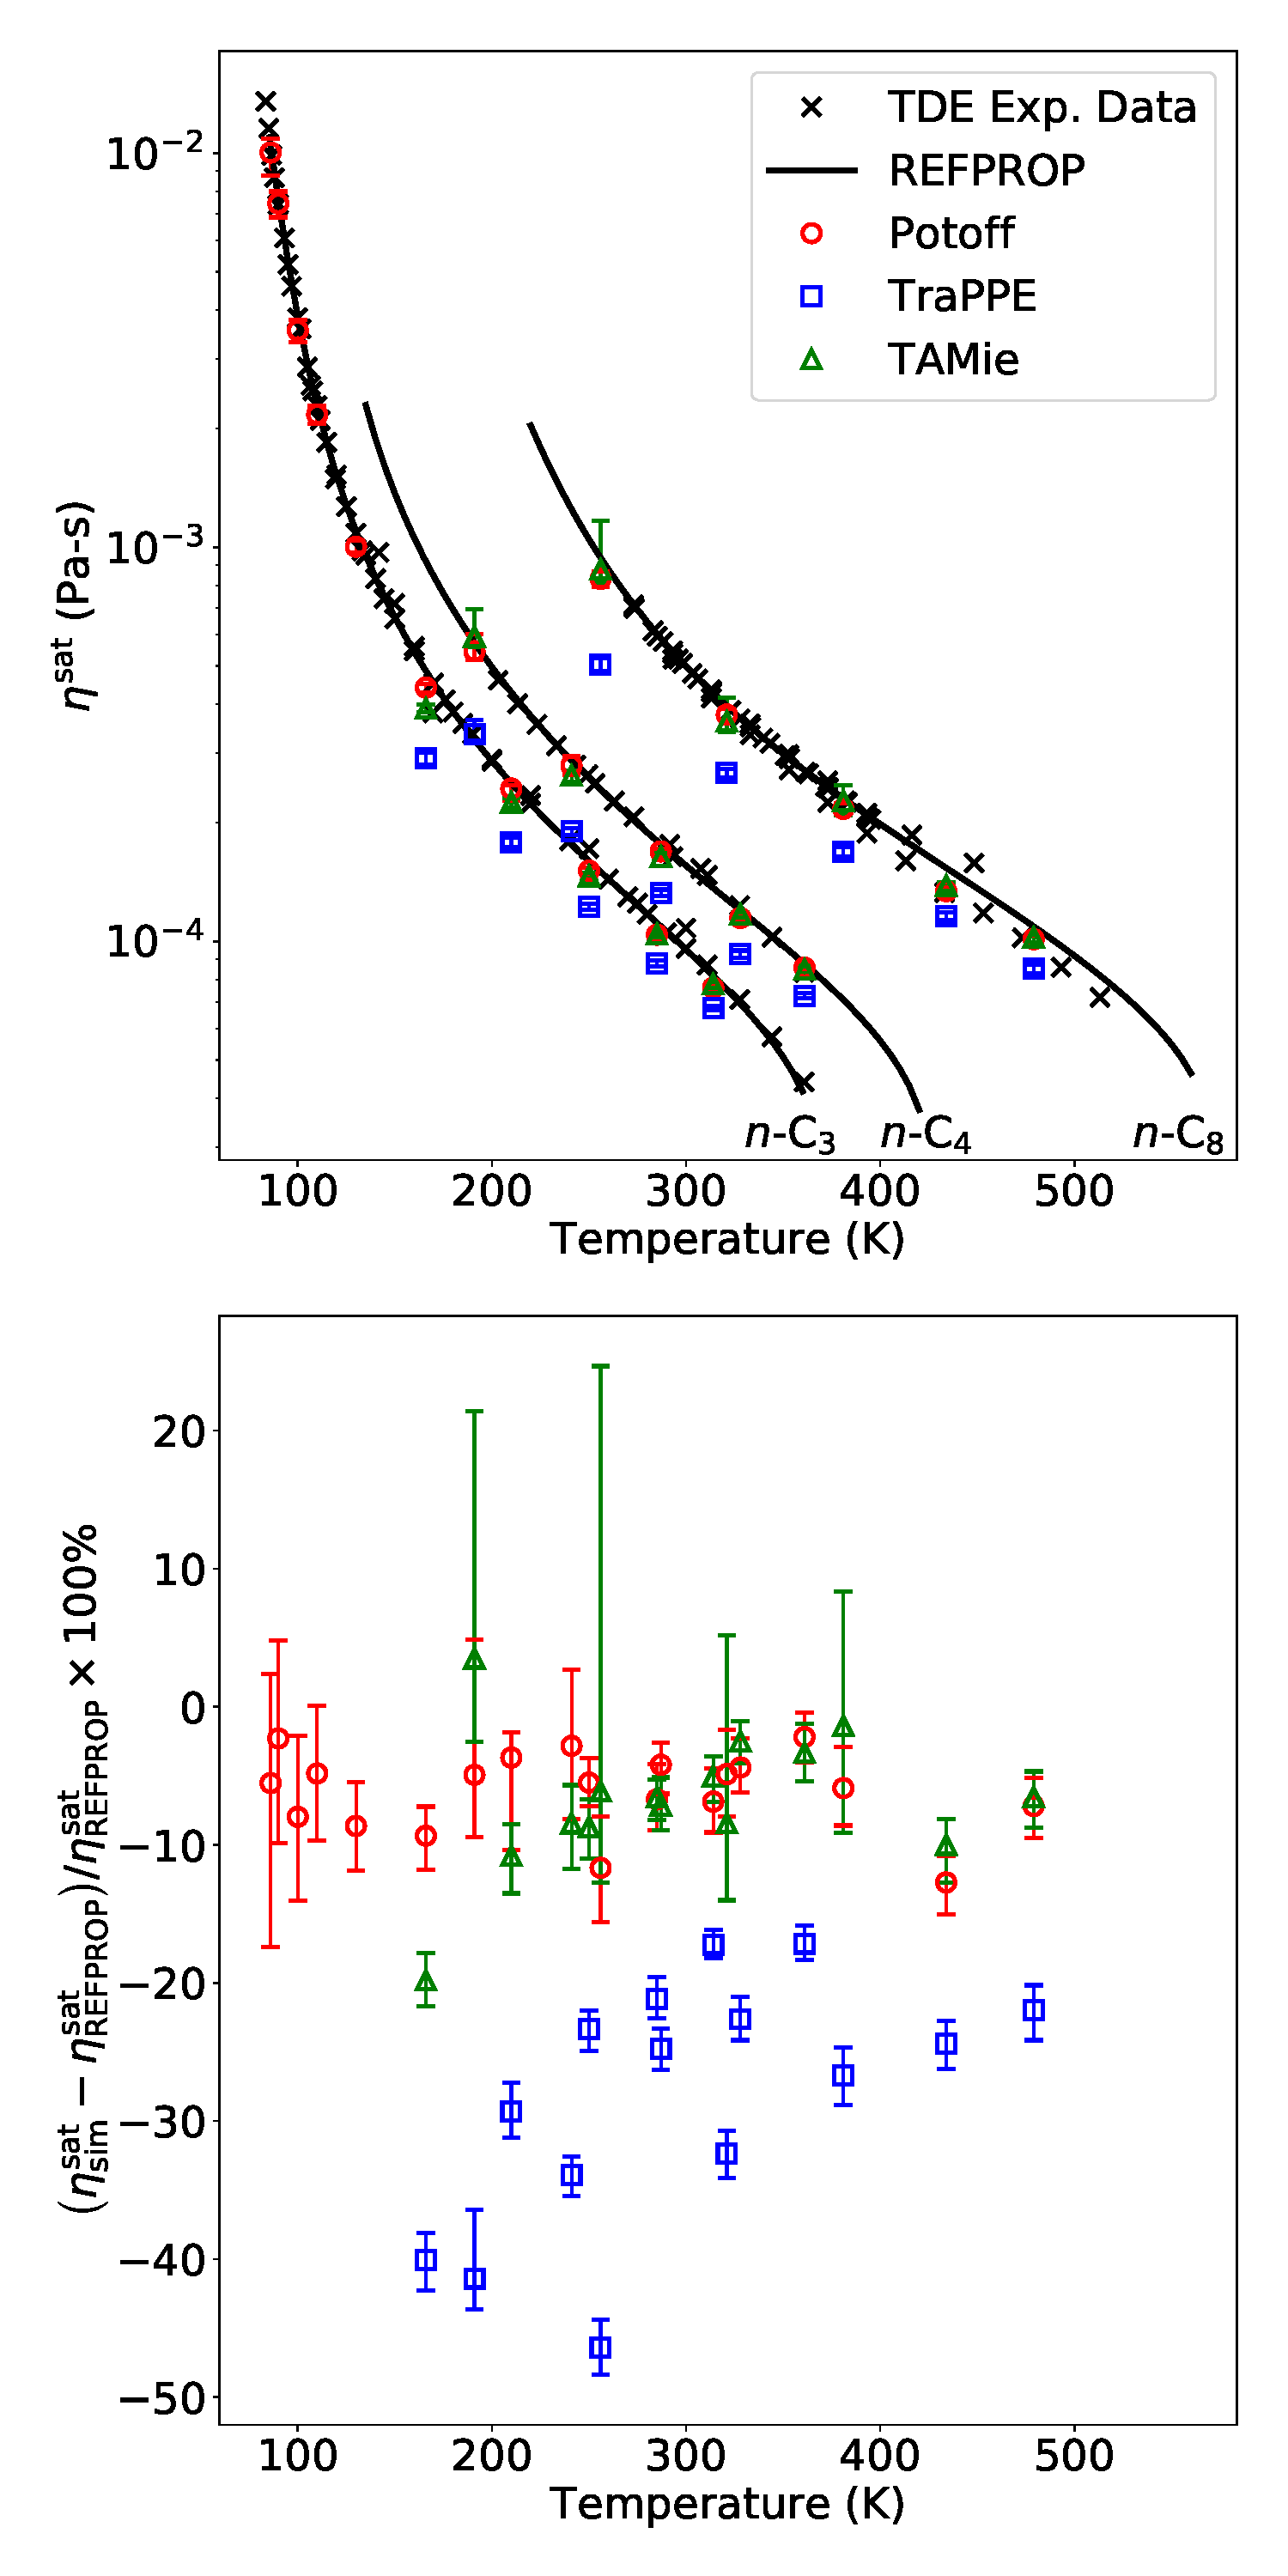
\includegraphics[width=3.2in]{compare_force_fields_alkanes.pdf}
		\caption{Saturated liquid viscosities for propane, \textit{n}-butane, and \textit{n}-octane. Colors/symbols denote different force fields.}
		\label{fig:Saturation_C3_C4_C8}
	\end{figure} 
	
	Figure \ref{fig:Saturation_C12_C16} compares the TraPPE, Potoff, and TAMie saturated liquid viscosities for \textit{n}-dodecane and \textit{n}-hexadecane. Although the TAMie and TraPPE results for these compounds are similar to those observed in Figure \ref{fig:Saturation_C3_C4_C8}, it is quite surprising that the Potoff results are nearly identical to the TraPPE results (which significantly under predict $\eta^{\rm sat}$). 
	
	\begin{figure}[p!]
		\centering
		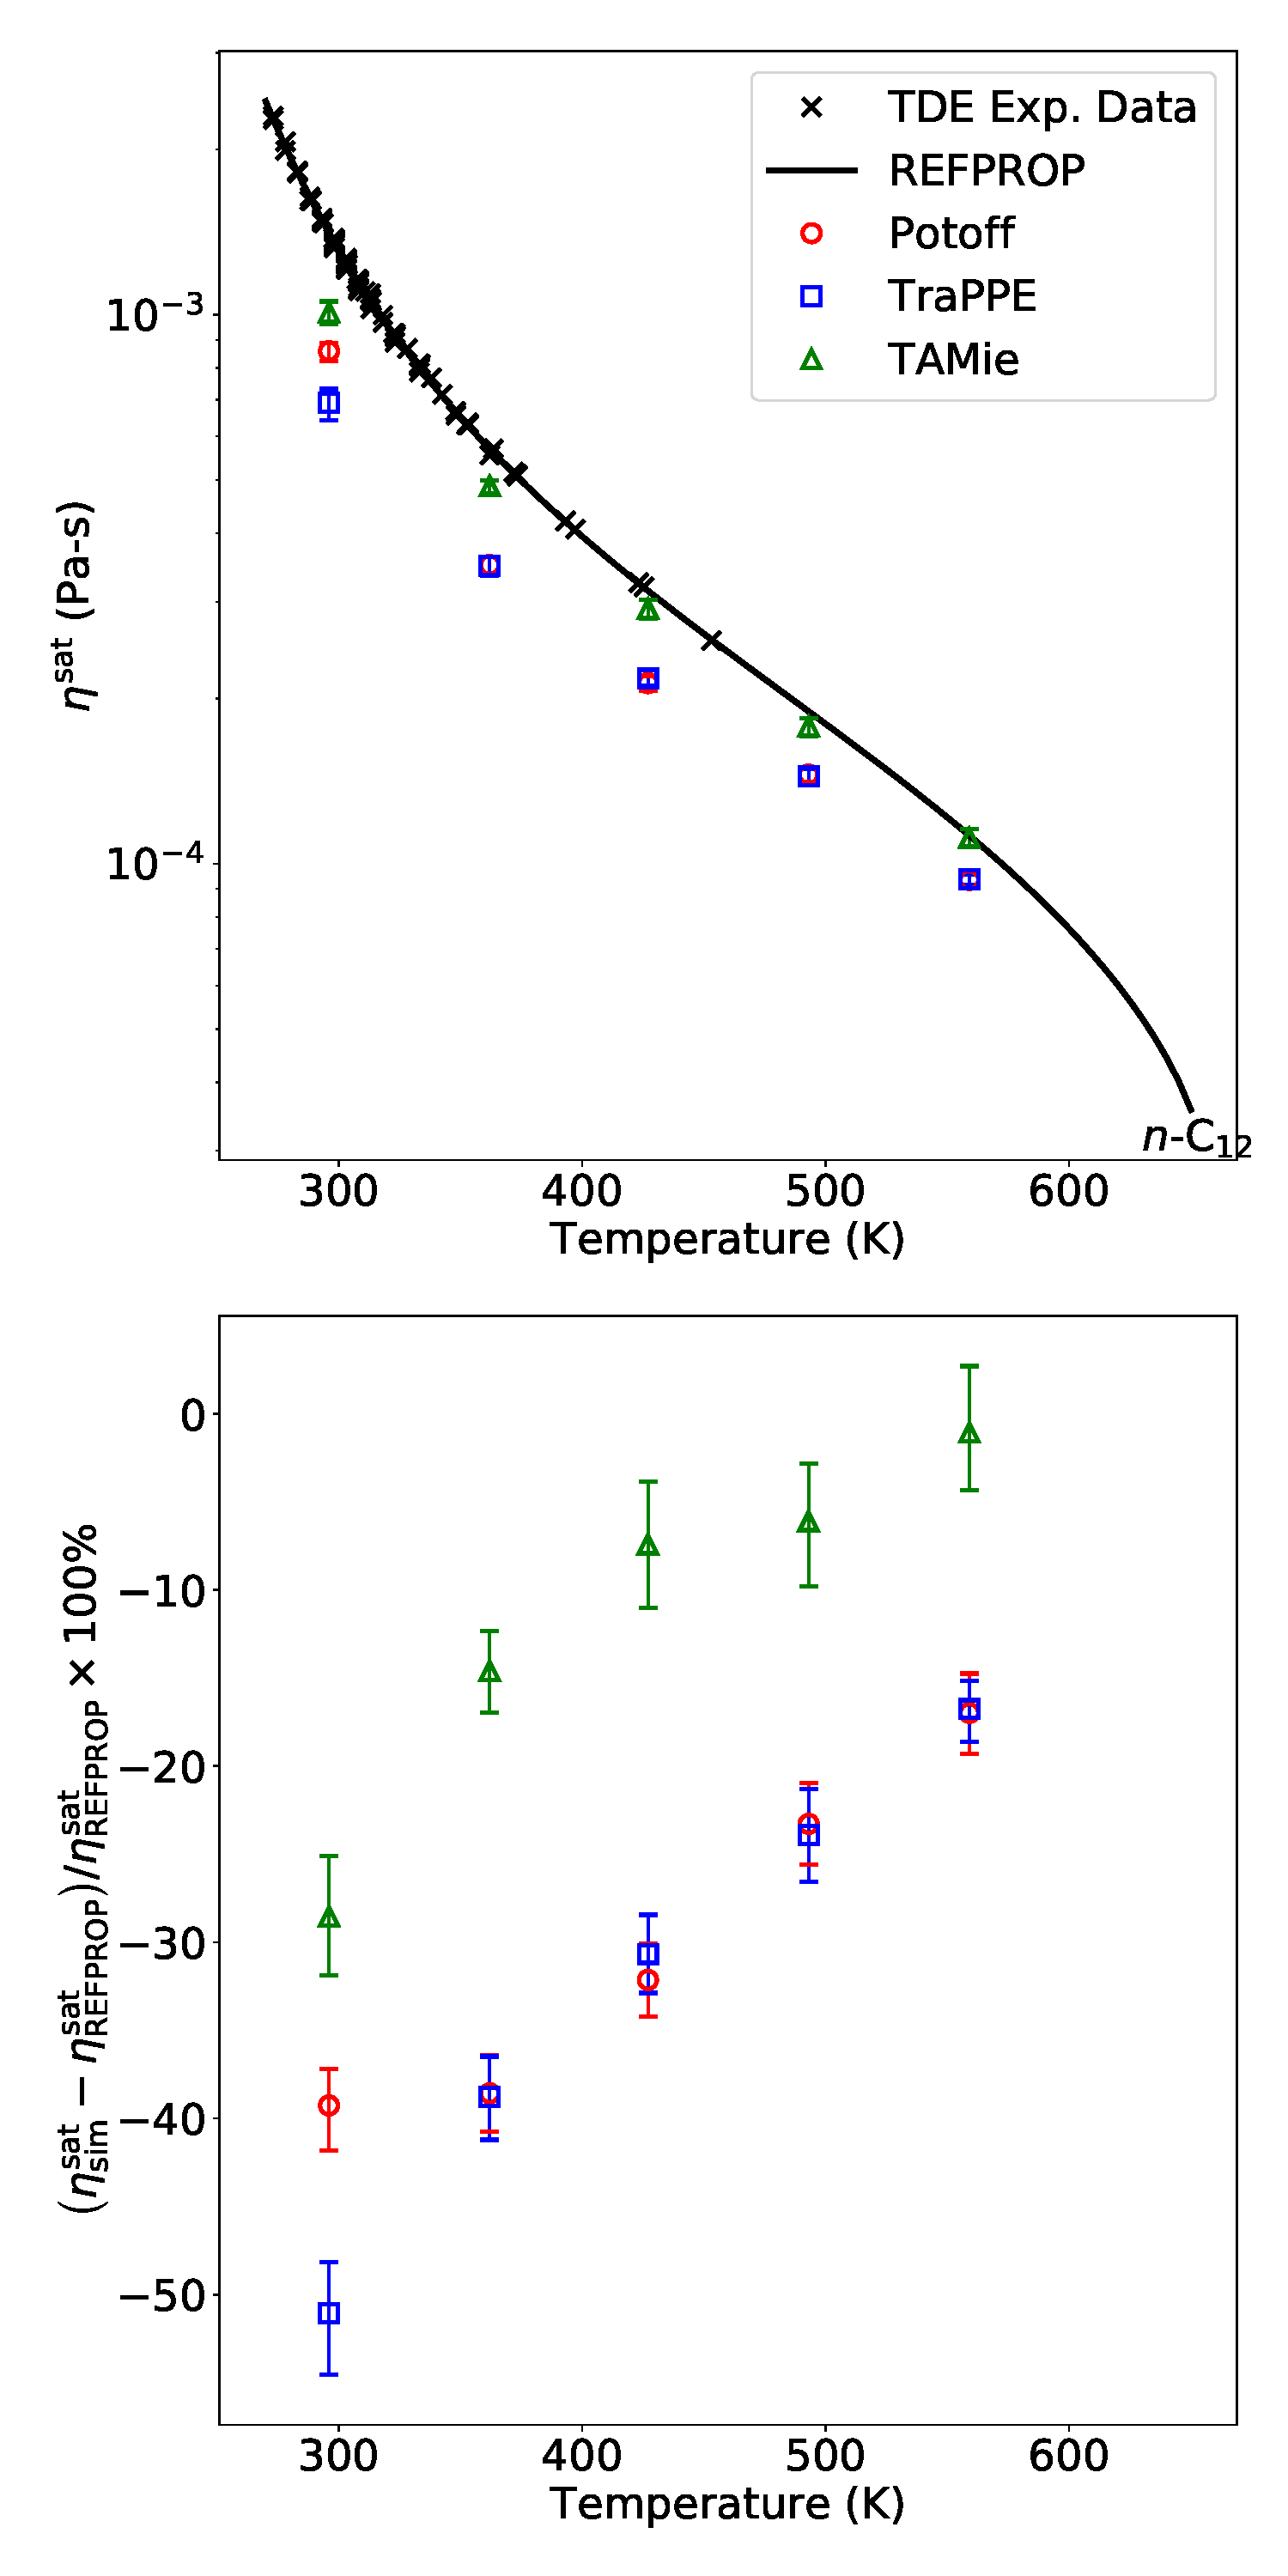
\includegraphics[width=3.2in]{compare_force_fields_C12.pdf}
		\caption{Saturated liquid viscosities for \textit{n}-dodecane and \textit{n}-hexadecane. Colors/symbols denote different force fields.}
		\label{fig:Saturation_C12_C16}
	\end{figure} 
	
	\subsubsection{Branched alkanes}
	
	%\begin{enumerate}
	%	\item Mie potential provides less improvement in these cases
	%\end{enumerate}
	
	%Figures:
	%
	%\begin{enumerate}
	%	\item IC4, NEOC5
	%	\item IC5, IC8
	%	\item IC6, 23DMB, 3MP
	%\end{enumerate}
	
	%Unfortunately, TAMie does not have parameters for C and, therefore, 
	
	%Figures \ref{fig:Saturation_IC4_NEOC5} to \ref{fig:Saturation_IC6_23DMB_3MP} compare the saturated liquid viscosities for each force field and branched alkane studied. Figure \ref{fig:Saturation_IC4_NEOC5} presents results for the more spherical compounds, namely, 2-methylpropane and 2,3-dimethylpropane. Figure \ref{fig:Saturation_IC5_IC8} presents results for a short and long chain, namely, 2-methylbutane and 2,2,4-trimethylpentane. Figure \ref{fig:Saturation_IC6_23DMB_3MP} presents results for various hexane isomers, namely, 2-methylpentane, 2,3-dimethylbutane, and 3-methylpentane. Each compound was simulated using the TraPPE (UA LJ 12-6) and Potoff (UA Mie 16-6) force fields. However, only 2-methylpropane and 2,3-dimethylpropane were simulated with AUA4 (AUA LJ 12-6) while 2,3-dimethylpropane and 2,2,4-trimethylpentane were not simulated using the TAMie (AUA Mie 14-6) force field.
	%
	%From Figure \ref{fig:Saturation_IC4_NEOC5} to \ref{fig:Saturation_IC6_23DMB_3MP}, we see that the Potoff S/L force field is not as accurate for the simulated branched alkanes as for the normal alkanes. However, it still provides considerable improvement compared to the LJ 12-6 based models, i.e., TraPPE and AUA4. Surprisingly, the TAMie force field performs much worse for these branched alkanes. 
	%
	%%Figure \ref{fig:Saturation_IC4_NEOC5} compares the TraPPE (UA LJ 12-6), AUA4 (AUA LJ 12-6), and Potoff (UA Mie 16-6) saturated liquid viscosities for 2-methylpropane and 2,3-dimethylpropane.
	%
	%\begin{figure}[p!]
	%	\centering
	%	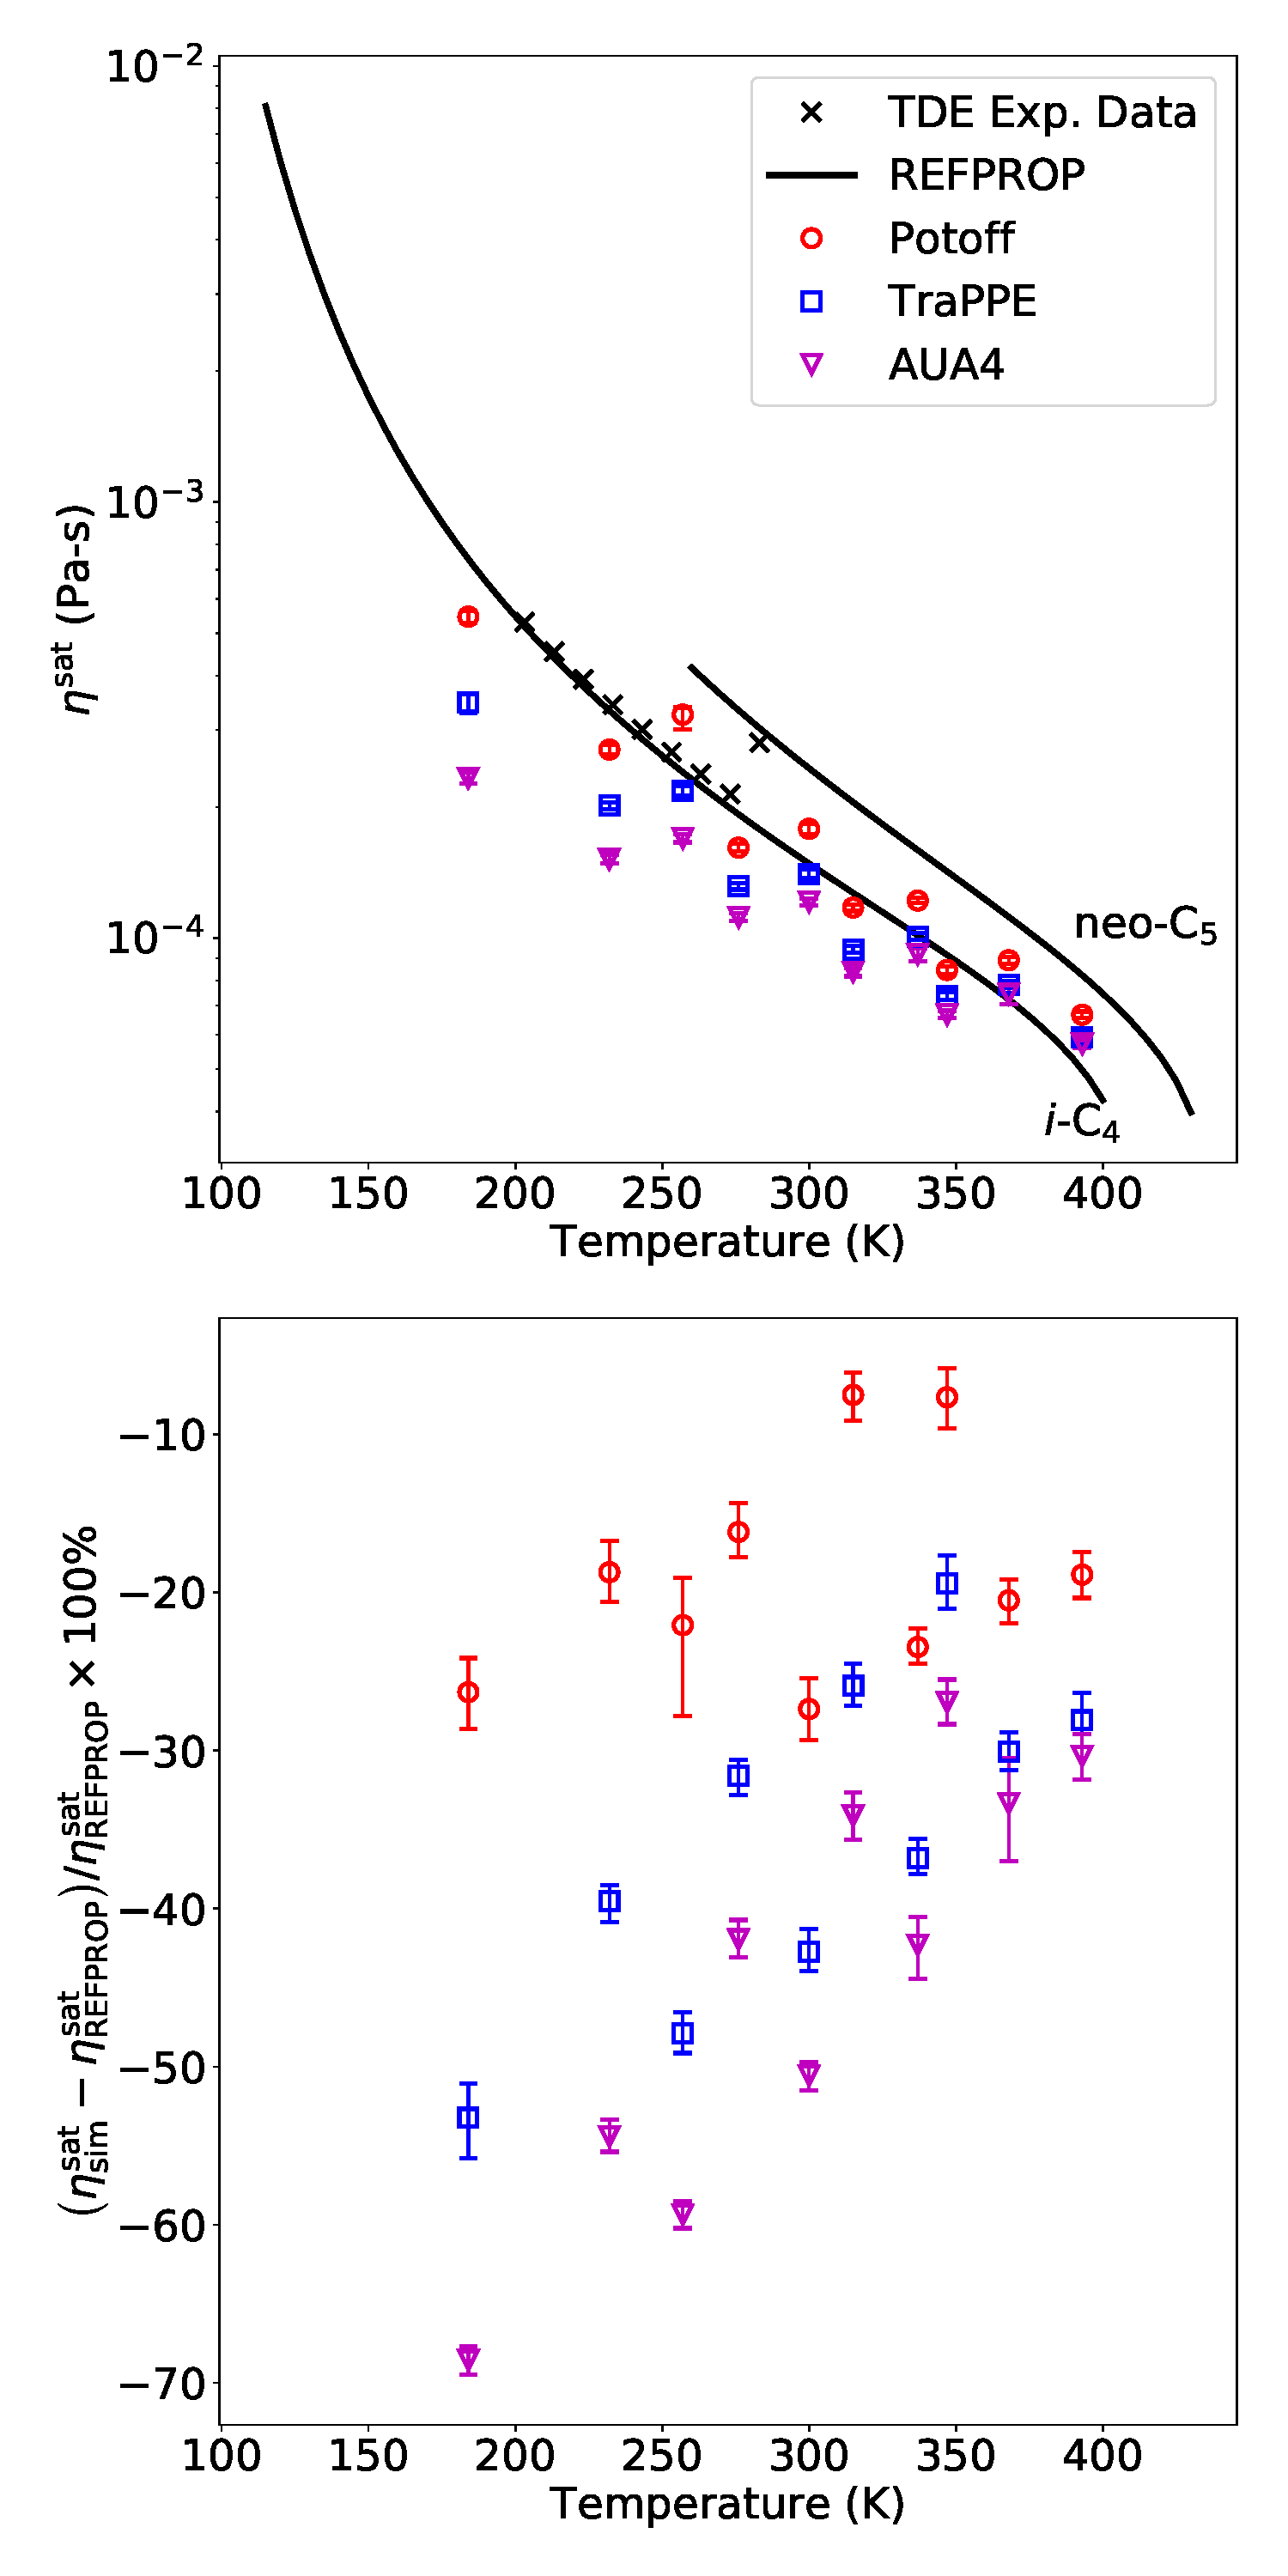
\includegraphics[width=3.2in]{compare_force_fields_IC4_neoC5.pdf}
	%	\caption{Saturated liquid viscosities for 2-methylpropane and 2,3-dimethylpropane. Colors/symbols denote different force fields.}
	%	\label{fig:Saturation_IC4_NEOC5}
	%\end{figure} 
	%
	%%Figure \ref{fig:Saturation_IC5_IC8} compares the TraPPE, Potoff, and TAMie saturated liquid viscosities for 2-methylbutane and 2,2,4-trimethylpentane.
	%
	%\begin{figure}[p!]
	%	\centering
	%	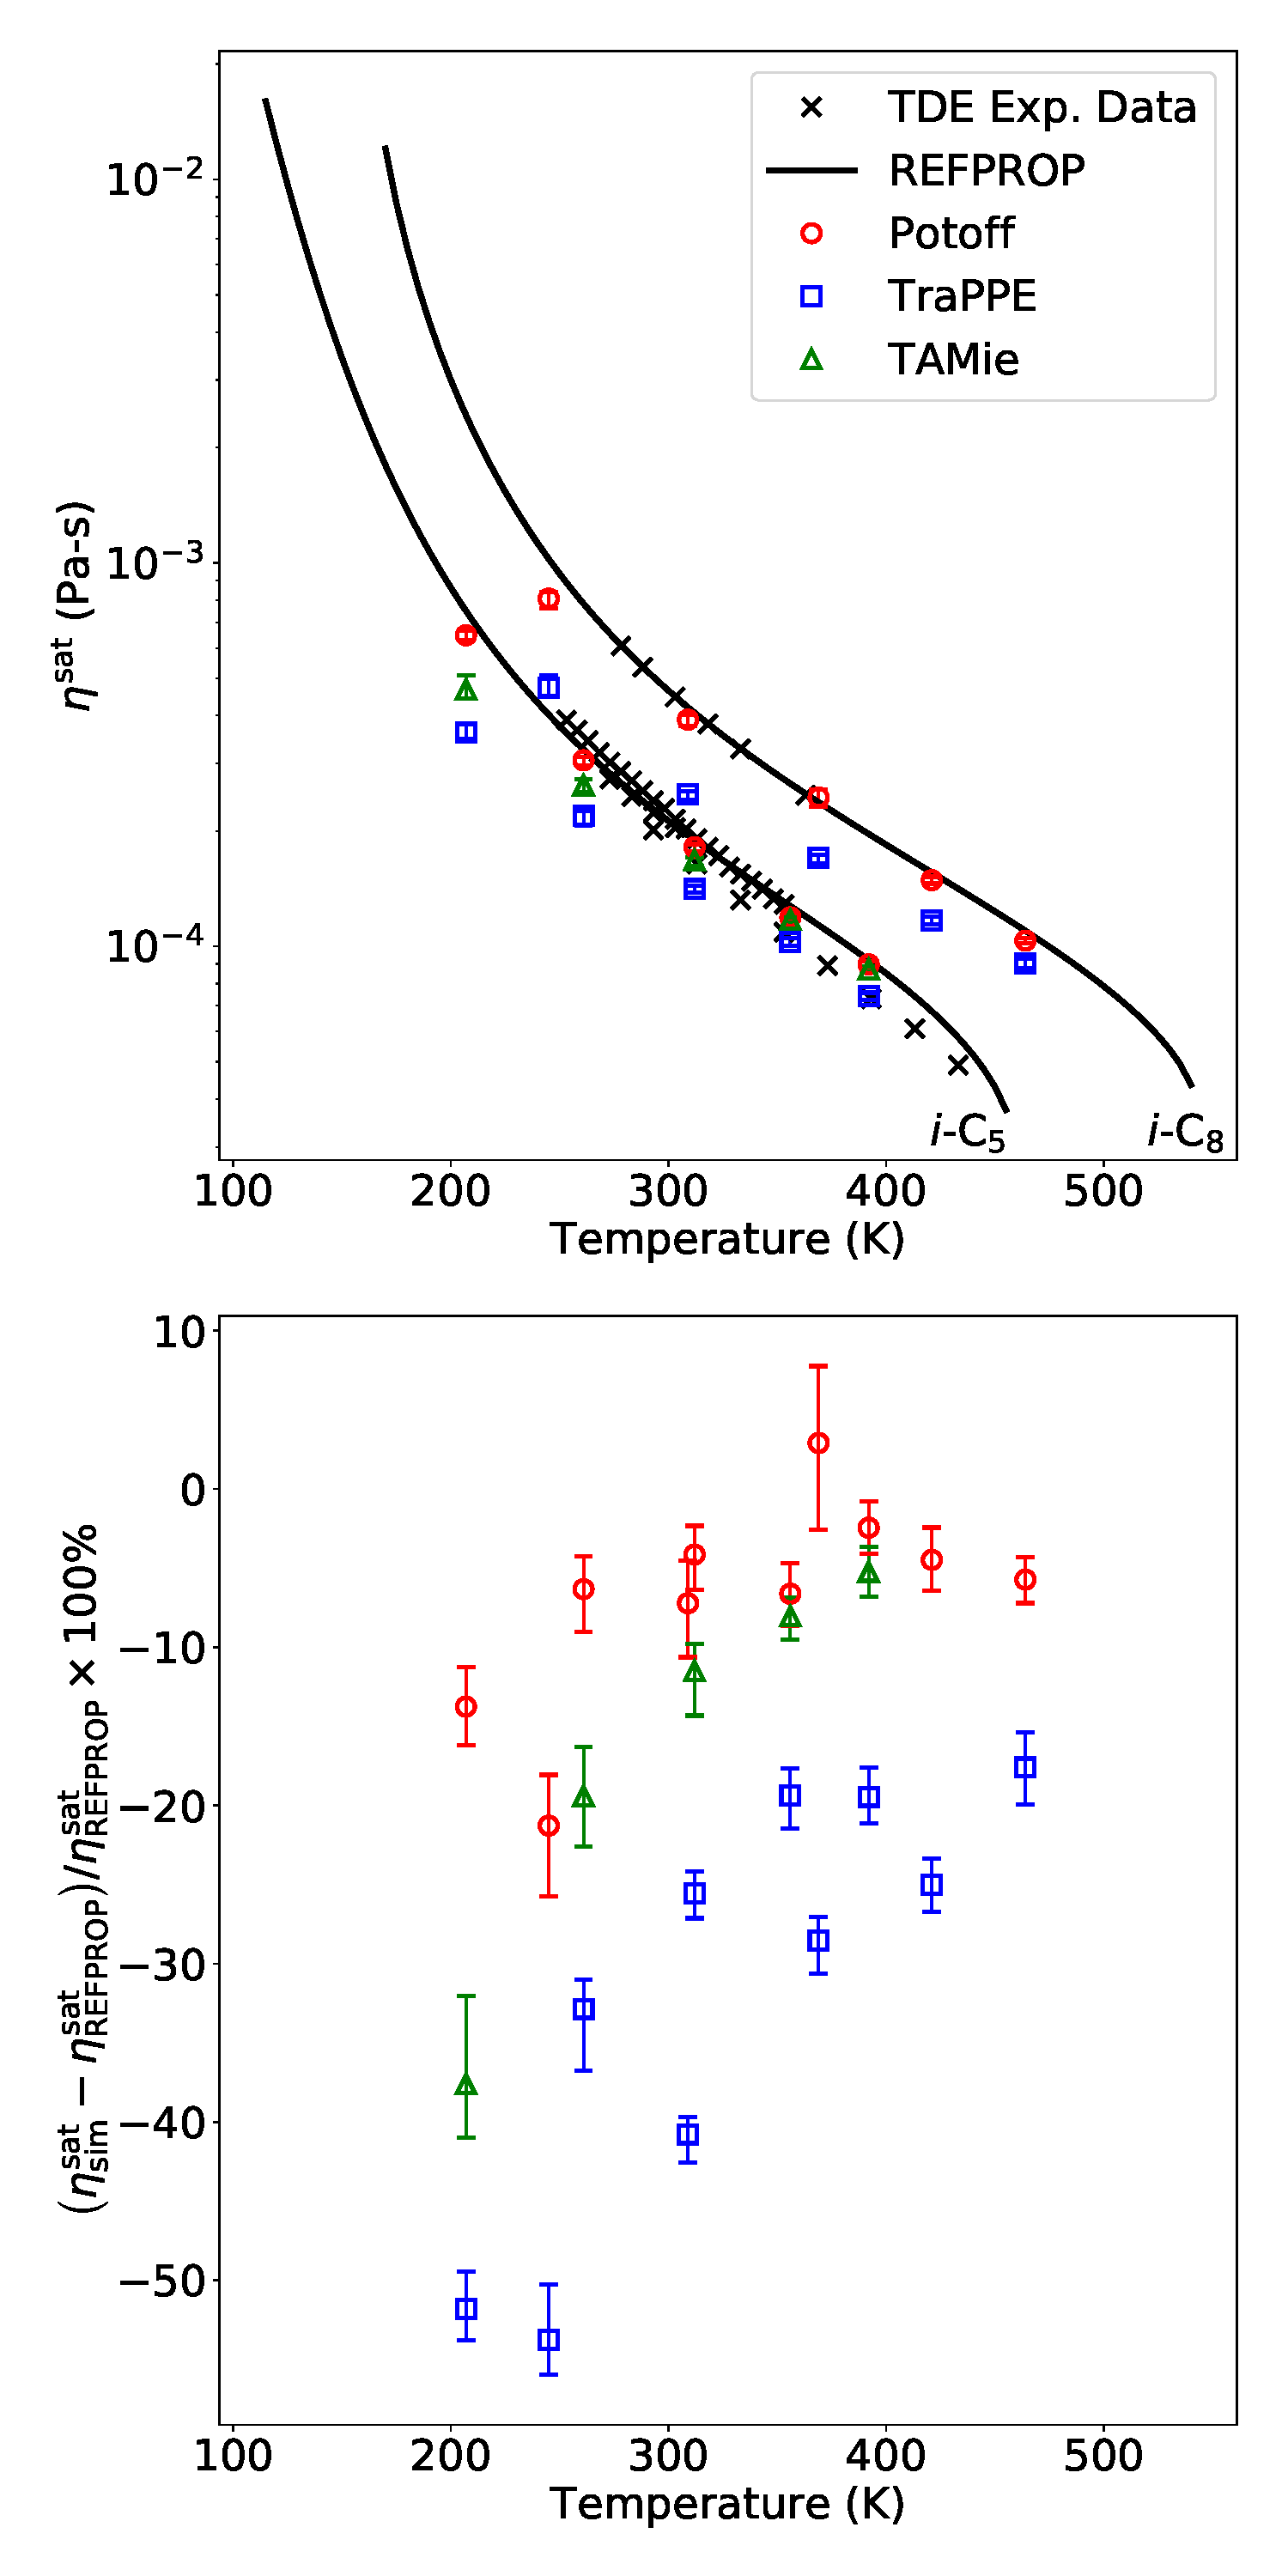
\includegraphics[width=3.2in]{compare_force_fields_IC5_IC8.pdf}
	%	\caption{Saturated liquid viscosities for 2-methylbutane and 2,2,4-trimethylpentane. Colors/symbols denote different force fields.}
	%	\label{fig:Saturation_IC5_IC8}
	%\end{figure} 
	%
	%%Figure \ref{fig:Saturation_IC6_23DMB_3MP} compares the TraPPE, Potoff, and TAMie saturated liquid viscosities for 2-methylbutane and 2,2,4-trimethylpentane.
	%
	%\begin{figure}[p!]
	%	\centering
	%	
\includegraphics[width=3.2in]{empty_figure.jpg}
	%	\caption{Saturated liquid viscosities for 2-methylpentane, 2,3-dimethylbutane, and 3-methylpentane. Colors/symbols denote different force fields.}
	%	\label{fig:Saturation_IC6_23DMB_3MP}
	%\end{figure}
	
	Figures \ref{fig:Saturation_short_branched} and \ref{fig:Saturation_long_branched} compare the saturated liquid viscosities for each force field and branched alkane studied. Figures \ref{fig:Saturation_short_branched} and \ref{fig:Saturation_long_branched} present results for the compounds classified by Potoff as ``short'' and ``long'', respectively. Specifically, Figure \ref{fig:Saturation_short_branched} depicts 2-methylpropane, 2,2-dimethylpropane, 2-methylbutane, and 2,3-dimethylbutane, while Figure \ref{fig:Saturation_long_branched} contains 2-methylpentane, 3-methylpentane, and 2,2,4-trimethylpentane. Each compound was simulated using the TraPPE (UA LJ 12-6) and Potoff (UA Mie 16-6) force fields. However, only 2-methylpropane and 2,2-dimethylpropane were simulated with AUA4 (AUA LJ 12-6) while 2,2-dimethylpropane and 2,2,4-trimethylpentane were not simulated using the TAMie (AUA Mie 14-6) force field.
	
	%From Figure \ref{fig:Saturation_IC4_NEOC5} to \ref{fig:Saturation_IC6_23DMB_3MP}, we see that the Potoff S/L force field is not as accurate for the simulated branched alkanes as for the normal alkanes. However, it still provides considerable improvement compared to the LJ 12-6 based models, i.e., TraPPE and AUA4. Surprisingly, the TAMie force field performs much worse for these branched alkanes. 
	
	\begin{figure}[p!]
		\centering
		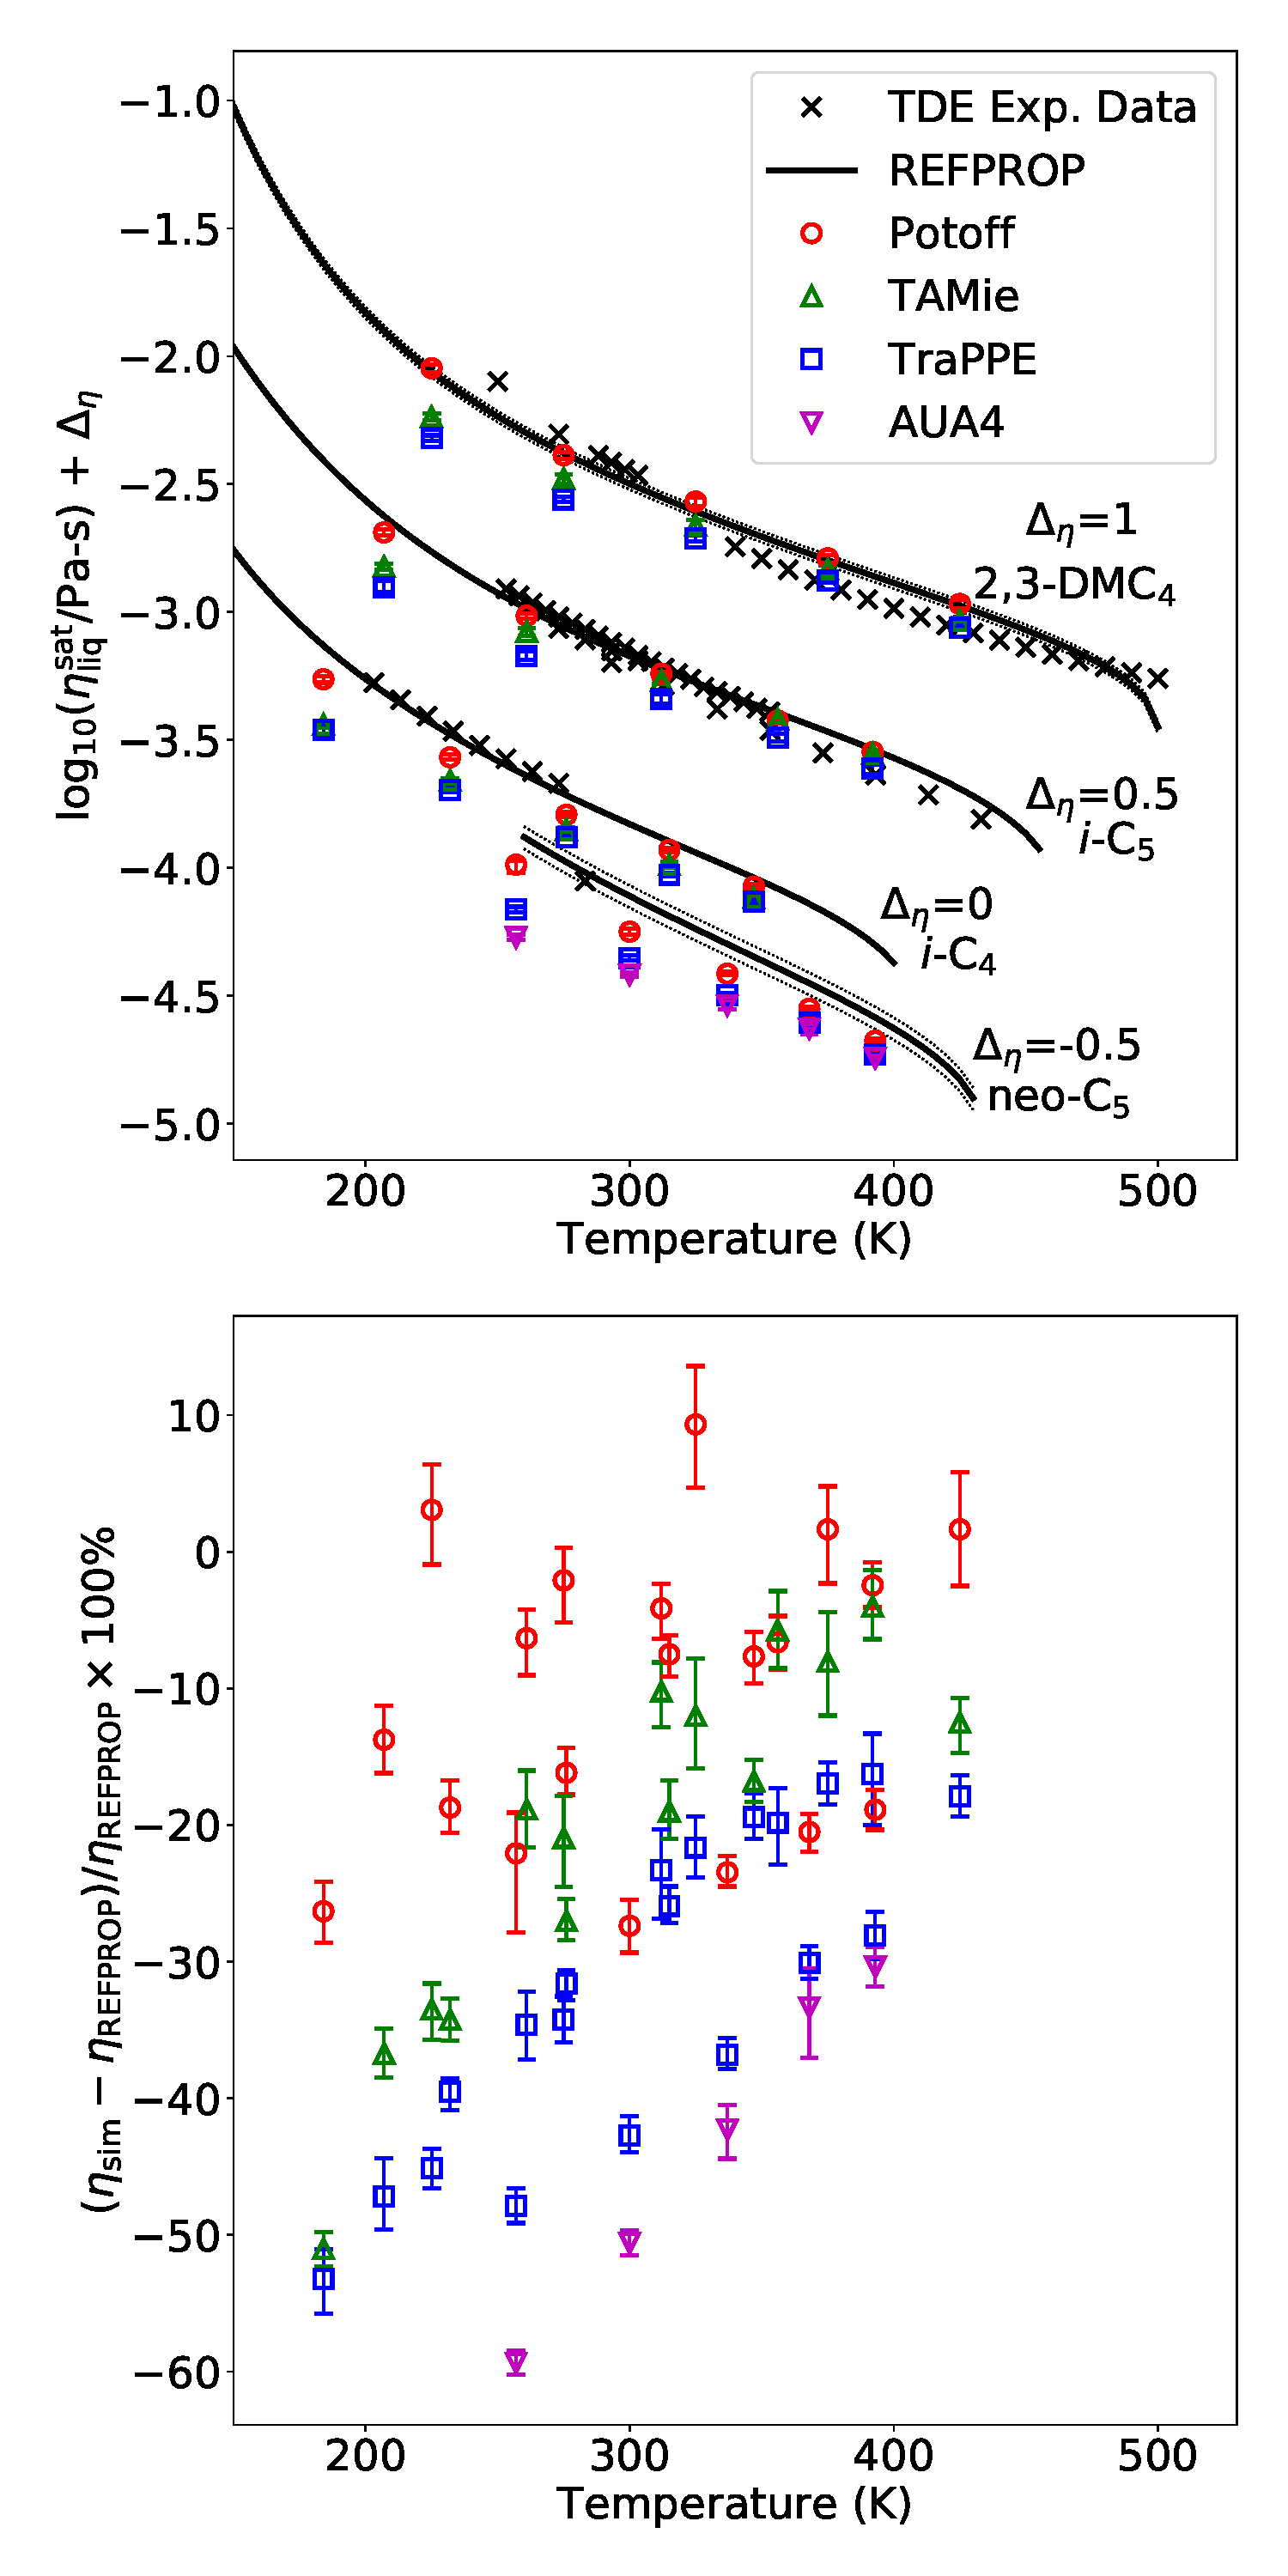
\includegraphics[width=3.2in]{compare_force_fields_short_branched.pdf}
		\caption{Saturated liquid viscosities for 2-methylpropane, 2,2-dimethylpropane, 2-methylbutane, and 2,3-dimethylbutane. Colors/symbols denote different force fields.}
		\label{fig:Saturation_short_branched}
	\end{figure} 
	
	\begin{figure}[p!]
		\centering
		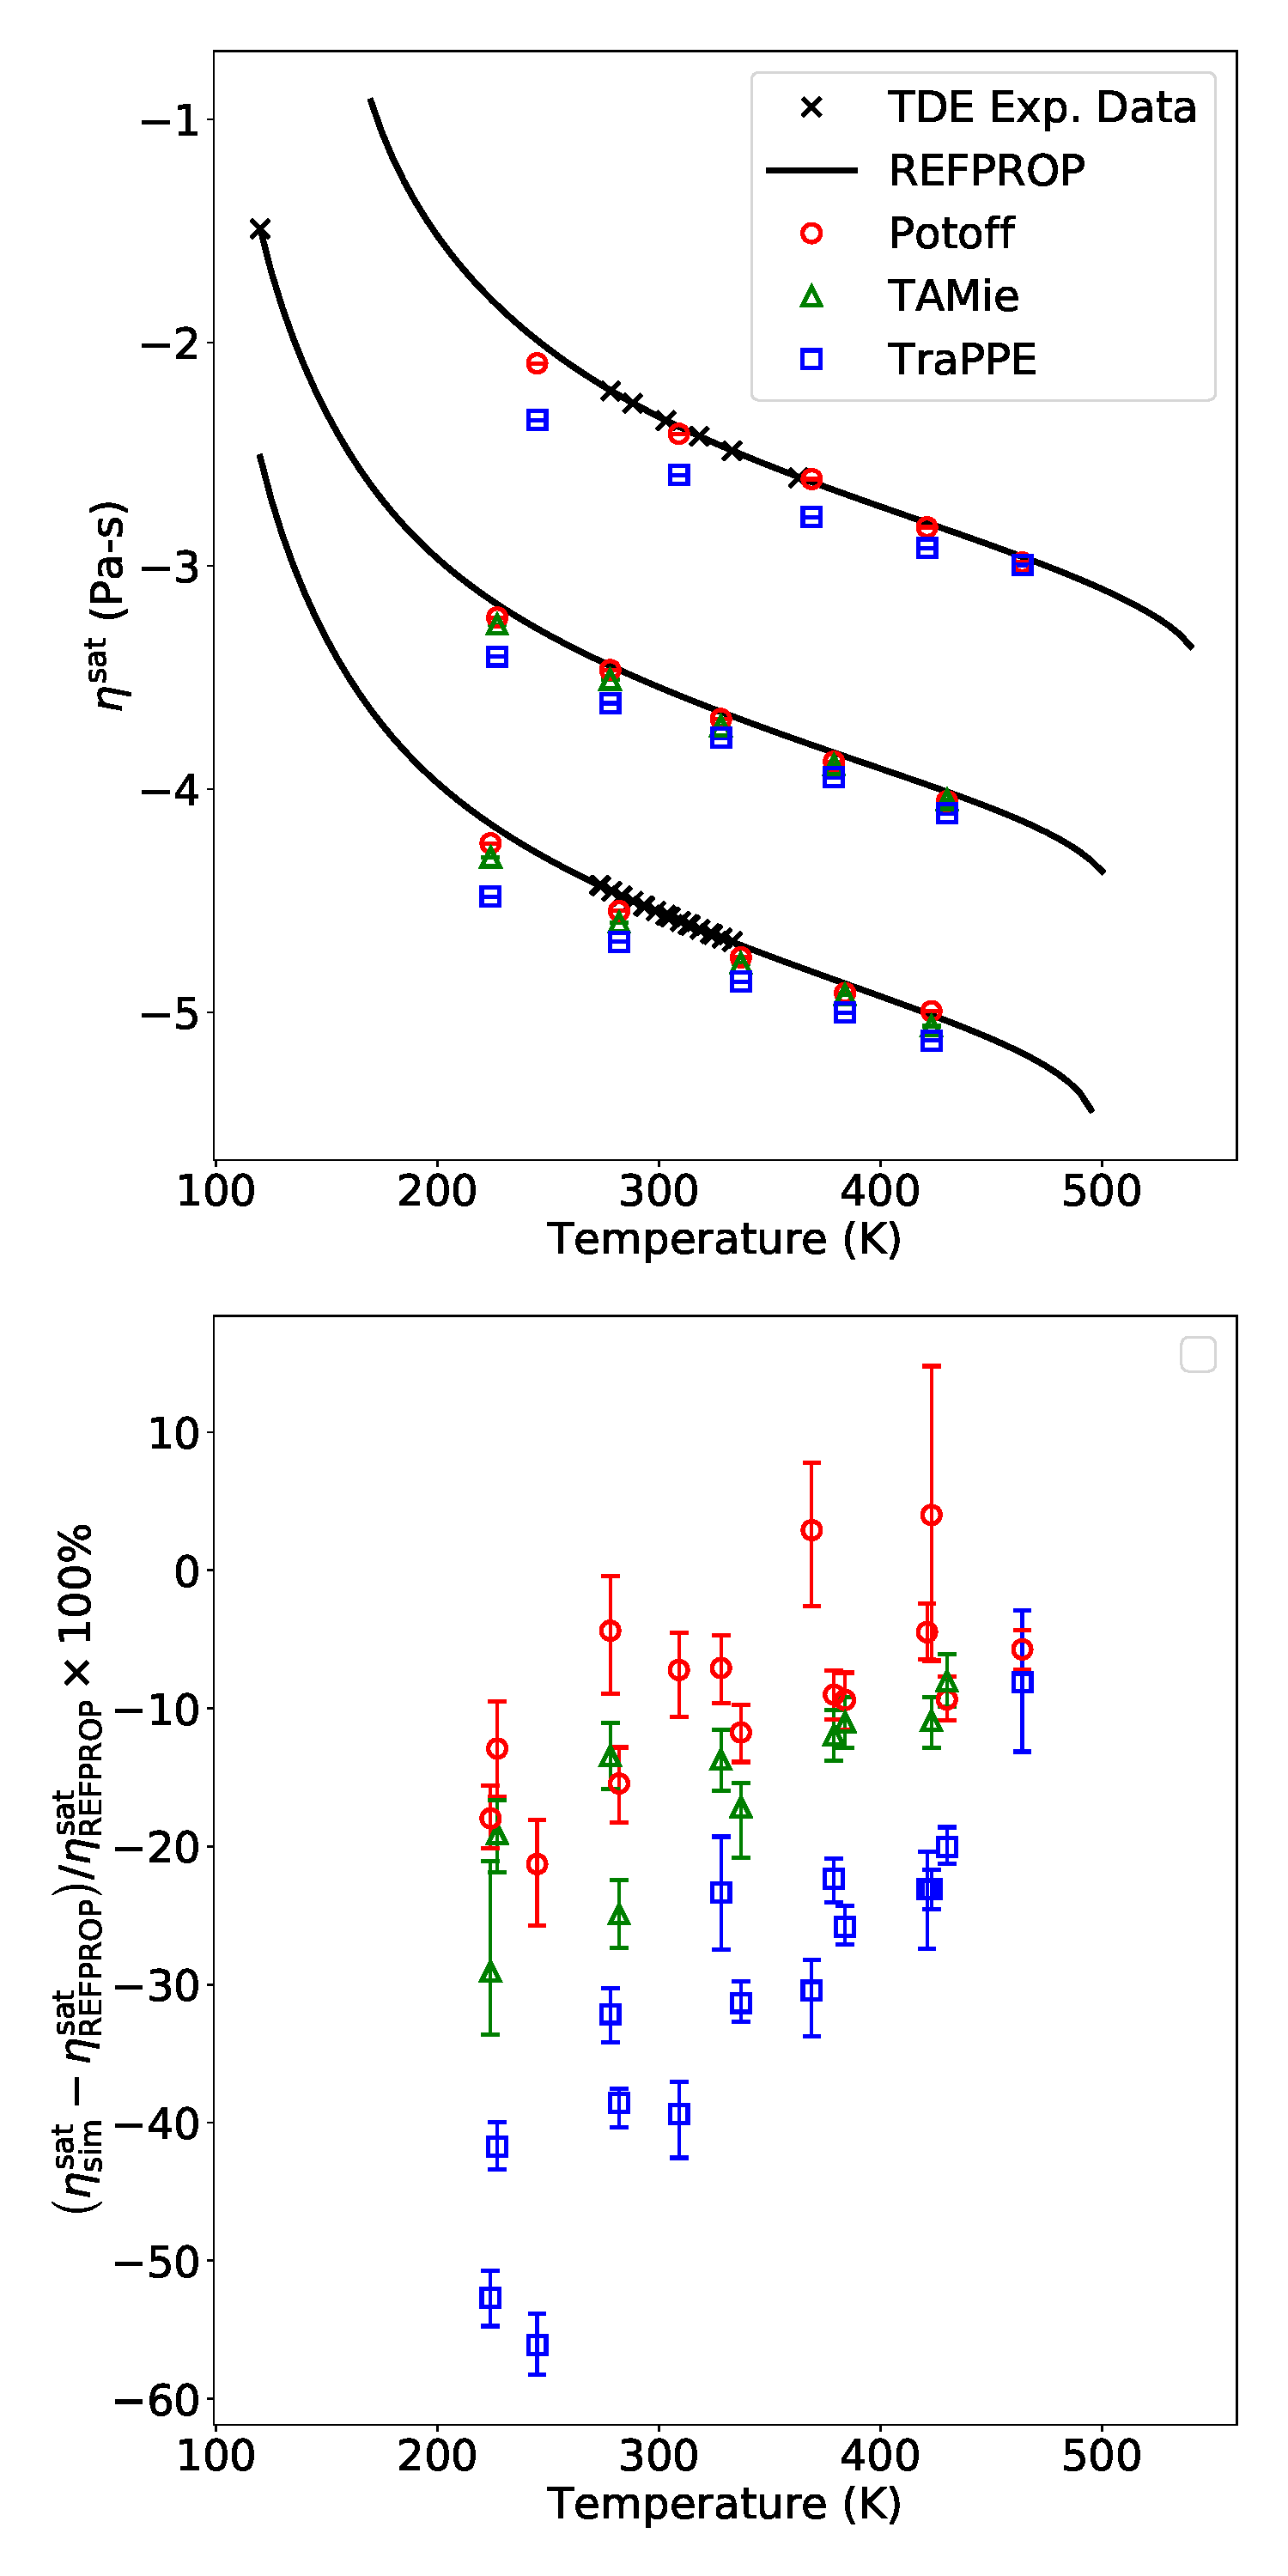
\includegraphics[width=3.2in]{compare_force_fields_long_branched.pdf}
		\caption{Saturated liquid viscosities for 2-methylpentane, 3-methylpentane, and 2,2,4-trimethylpentane. Colors/symbols denote different force fields.}
		\label{fig:Saturation_long_branched}
	\end{figure} 
	
	From Figures \ref{fig:Saturation_short_branched} and \ref{fig:Saturation_long_branched}, we see that the Potoff S/L and TAMie force fields are not as accurate for these branched alkanes as for the normal alkanes. In particular, Potoff and TAMie demonstrates the same temperature dependence observed for other force fields, where the deviations are largest at lower temperatures. However, Potoff still provides considerable improvement compared to the LJ 12-6 based models, i.e., TraPPE and AUA4. Note that the performance is similar for the Potoff ``short'' and ``long'' parameters in Figures \ref{fig:Saturation_short_branched} and \ref{fig:Saturation_long_branched}, respectively. 
	
	%The one apparent exception is 3-methylpentane, where the Potoff deviations are less than 10 \% over the entire temperature range. However, considering the availabi 
	
	The deviations for each force field are largest for 2-methylpropane and 2,2-dimethylpropane. Since these compounds are primarily composed of CH$_3$ UA sites, this poor performance is likely due to the assumption that the CH$_3$ non-bonded parameters are transferable from \textit{n}-alkanes to branched alkanes. Improvement might be possible if the CH$_3$ parameters were different depending on the neighboring UA site type.
	
	\subsection{High pressure fluid} \label{sec:T293highP}
	
	Section \ref{sec:eta_sat} demonstrated that Mie n-6 based force fields (Potoff and TAMie) are considerably more reliable for predicting saturated liquid viscosities than LJ 12-6 based force fields (TraPPE and AUA4). However, both the Potoff and TAMie non-bonded potentials use $n > 12$. Reference BLANK demonstrates that $n > 12$ leads to strong negative consequences at high densities/pressures. Specifically, $n > 12$ is too repulsive at short distances which leads to over estimates of pressure at high densities. For this reason, this section compares the different force fields above saturation pressure.
	
	\subsubsection{n-Alkanes}
	
	\begin{enumerate}
		\item Propane has accurate viscosity-P but not viscosity-rho
		\item Butane appears to agree more closely with recent REFPROP correlation
	\end{enumerate}
	
	%Figures:
	%
	%\begin{enumerate}
	%	\item Propane $\eta-\rho$ $\eta-P$
	%	\item Butane $\eta-\rho$ $\eta-P$
	%	\item n-Octane $\eta-\rho$ $\eta-P$
	%	%	\item n-Dodecane $\eta-\rho$ $\eta-P$?
	%\end{enumerate}
	
	Figures \ref{fig:T293highP_C3}, \ref{fig:T293highP_C4}, and \ref{fig:T293highP_C8} compare the elevated pressure viscosities for propane, \textit{n}-butane, and \textit{n}-octane, respectively. Each compound is simulated using the TraPPE, Potoff, and TAMie force fields. Note that for propane and \textit{n}-butane (Figures \ref{fig:T293highP_C3} and \ref{fig:T293highP_C4}) each force field is simulated at the same density, while for \textit{n}-octane (Figure \ref{fig:T293highP_C8}) the force fields are simulated at the same pressure. 
	
	%As the REFPROP viscosity correlation is not recommended above 100 MPa at 293 K, we have plotted some experimental data to guide the eye.
	
	Figure \ref{fig:T293highP_C3} demonstrates that the TraPPE force field has a constant negative bias even with increasing density/pressure. The TAMie force field has the most accurate $\eta$-$\rho$ dependence, i.e., the error does not increase with respect to density. By contrast, the Potoff potential demonstrates considerable over estimation of $\eta$ at high densities, which is likely attributed to the overly repulsive Mie 16-6 potential at close distances. Remarkably, the Potoff force field is the most accurate at predicting the $\eta$-$P$ dependence. This can be explained as a cancellation of errors since the Potoff force field significantly over predicts both viscosity and pressure at high densities. 
	
	The results in Figures \ref{fig:T293highP_C4} and \ref{fig:T293highP_C8} for \textit{n}-butane and \textit{n}-octane, respectively, are similar to those in Figure \ref{fig:T293highP_C3} for propane. Specifically, the TraPPE force field under predicts $\eta$ at all densities/pressures, the TAMie force field provides the most accurate $\eta$-$\rho$ dependence, while the Potoff force field over predicts $\eta$-$\rho$ dependence but accurately predicts the $\eta$-P dependence.  
	
	\begin{figure}[p!]
		\centering
		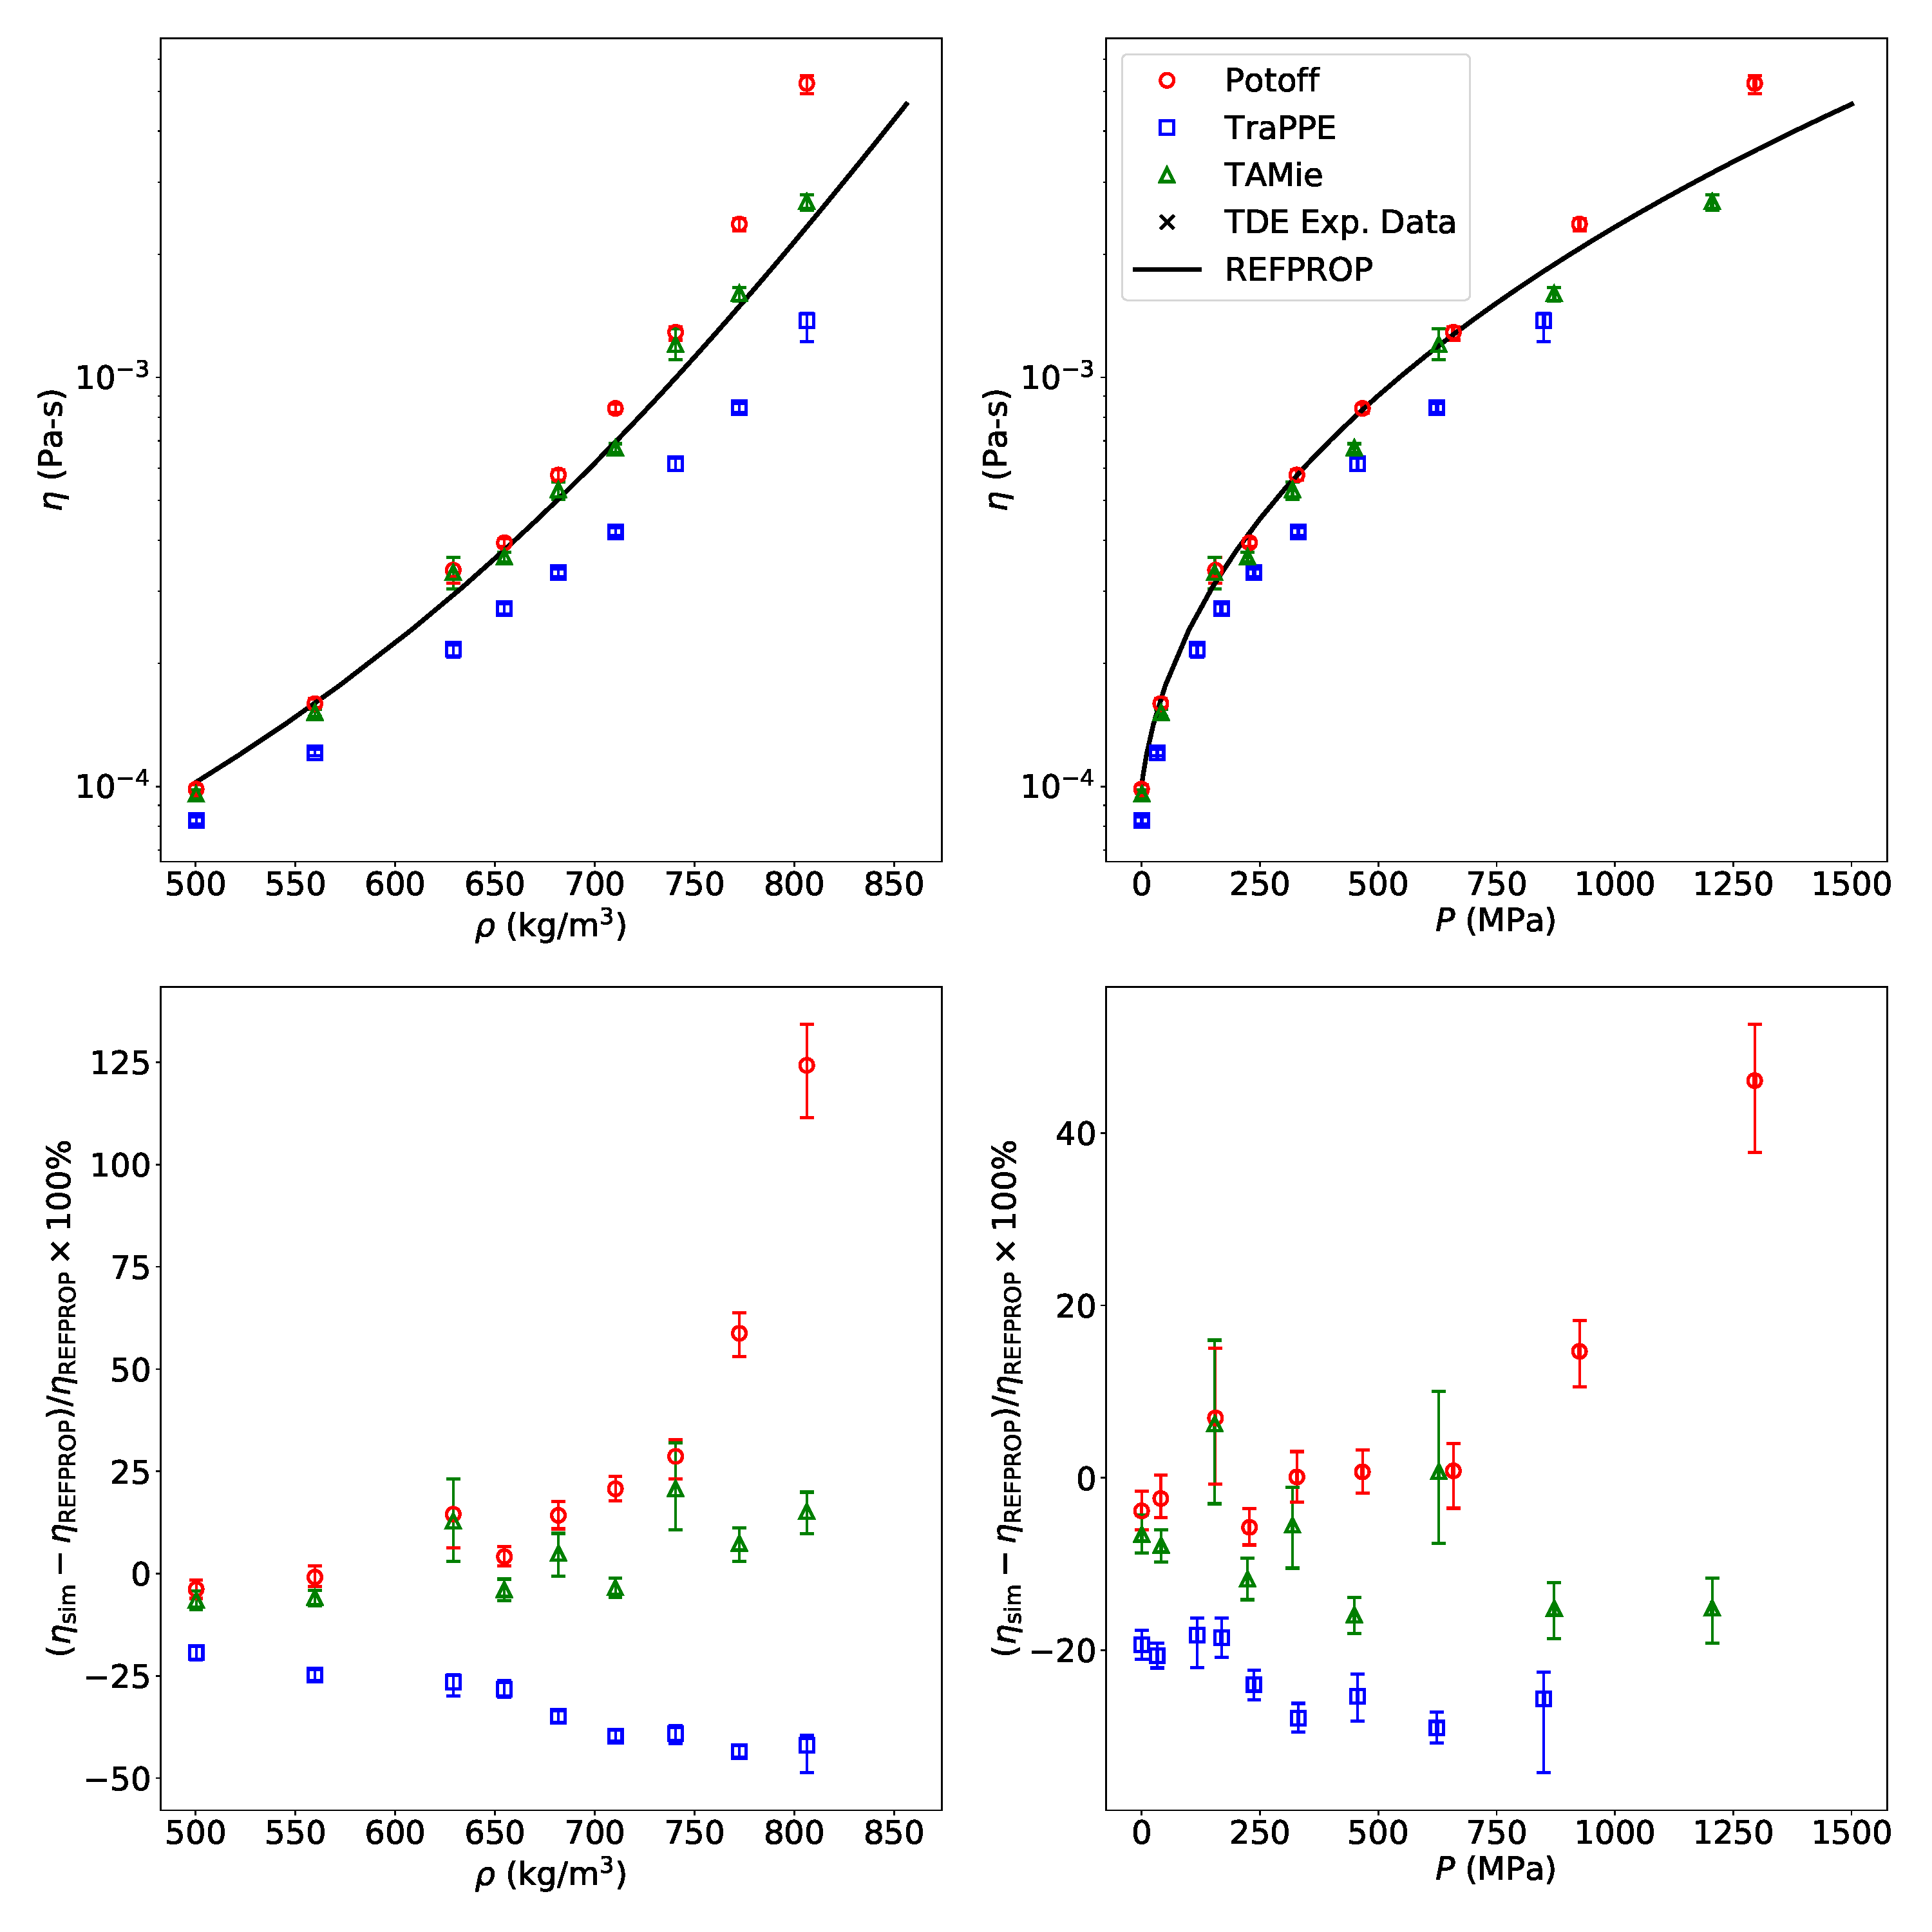
\includegraphics[width=6.4in]{compare_REFPROP_T293highP_C3H8_Pas.pdf}
		\caption{High density fluid viscosities at 293 K for propane. Colors/symbols denote different force fields.}
		\label{fig:T293highP_C3}
	\end{figure} 
	
	\begin{figure}[p!]
		\centering
		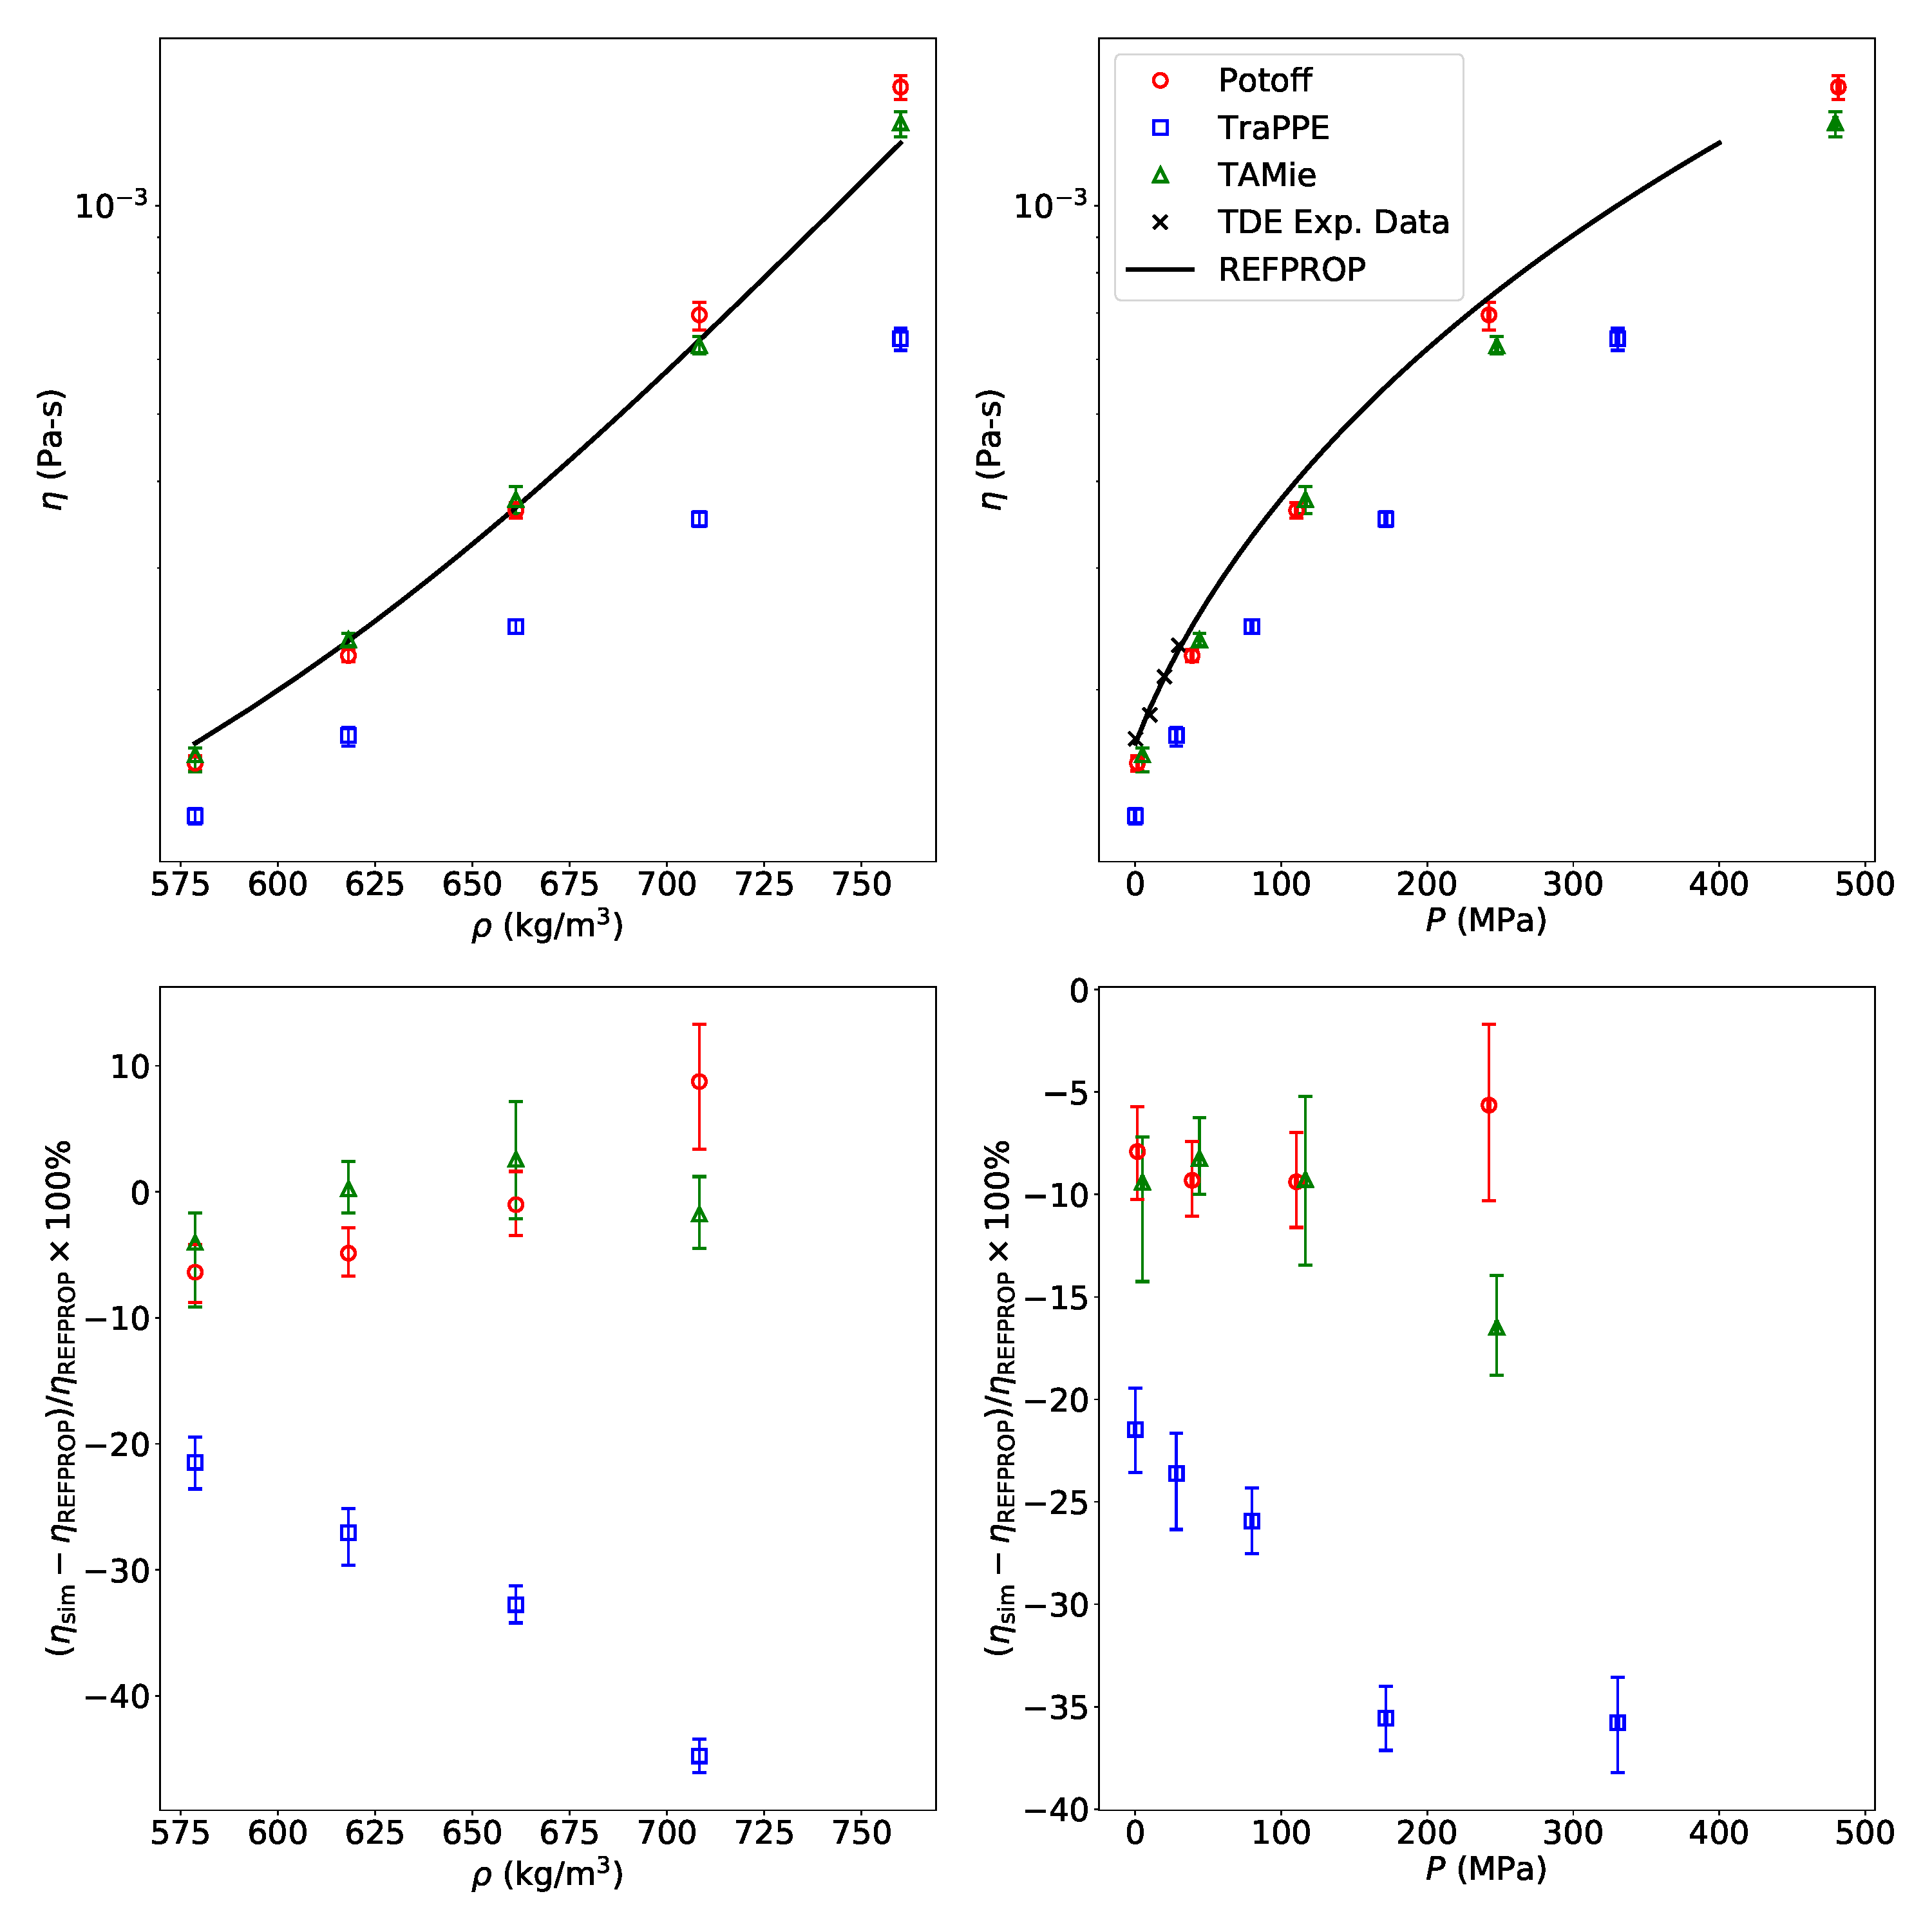
\includegraphics[width=6.4in]{compare_REFPROP_T293highP_C4H10_Pas_new_REFPROP.pdf}
		\caption{High density fluid viscosities at 293 K for \textit{n}-butane. Colors/symbols denote different force fields.}
		\label{fig:T293highP_C4}
	\end{figure} 
	
	\begin{figure}[p!]
		\centering
		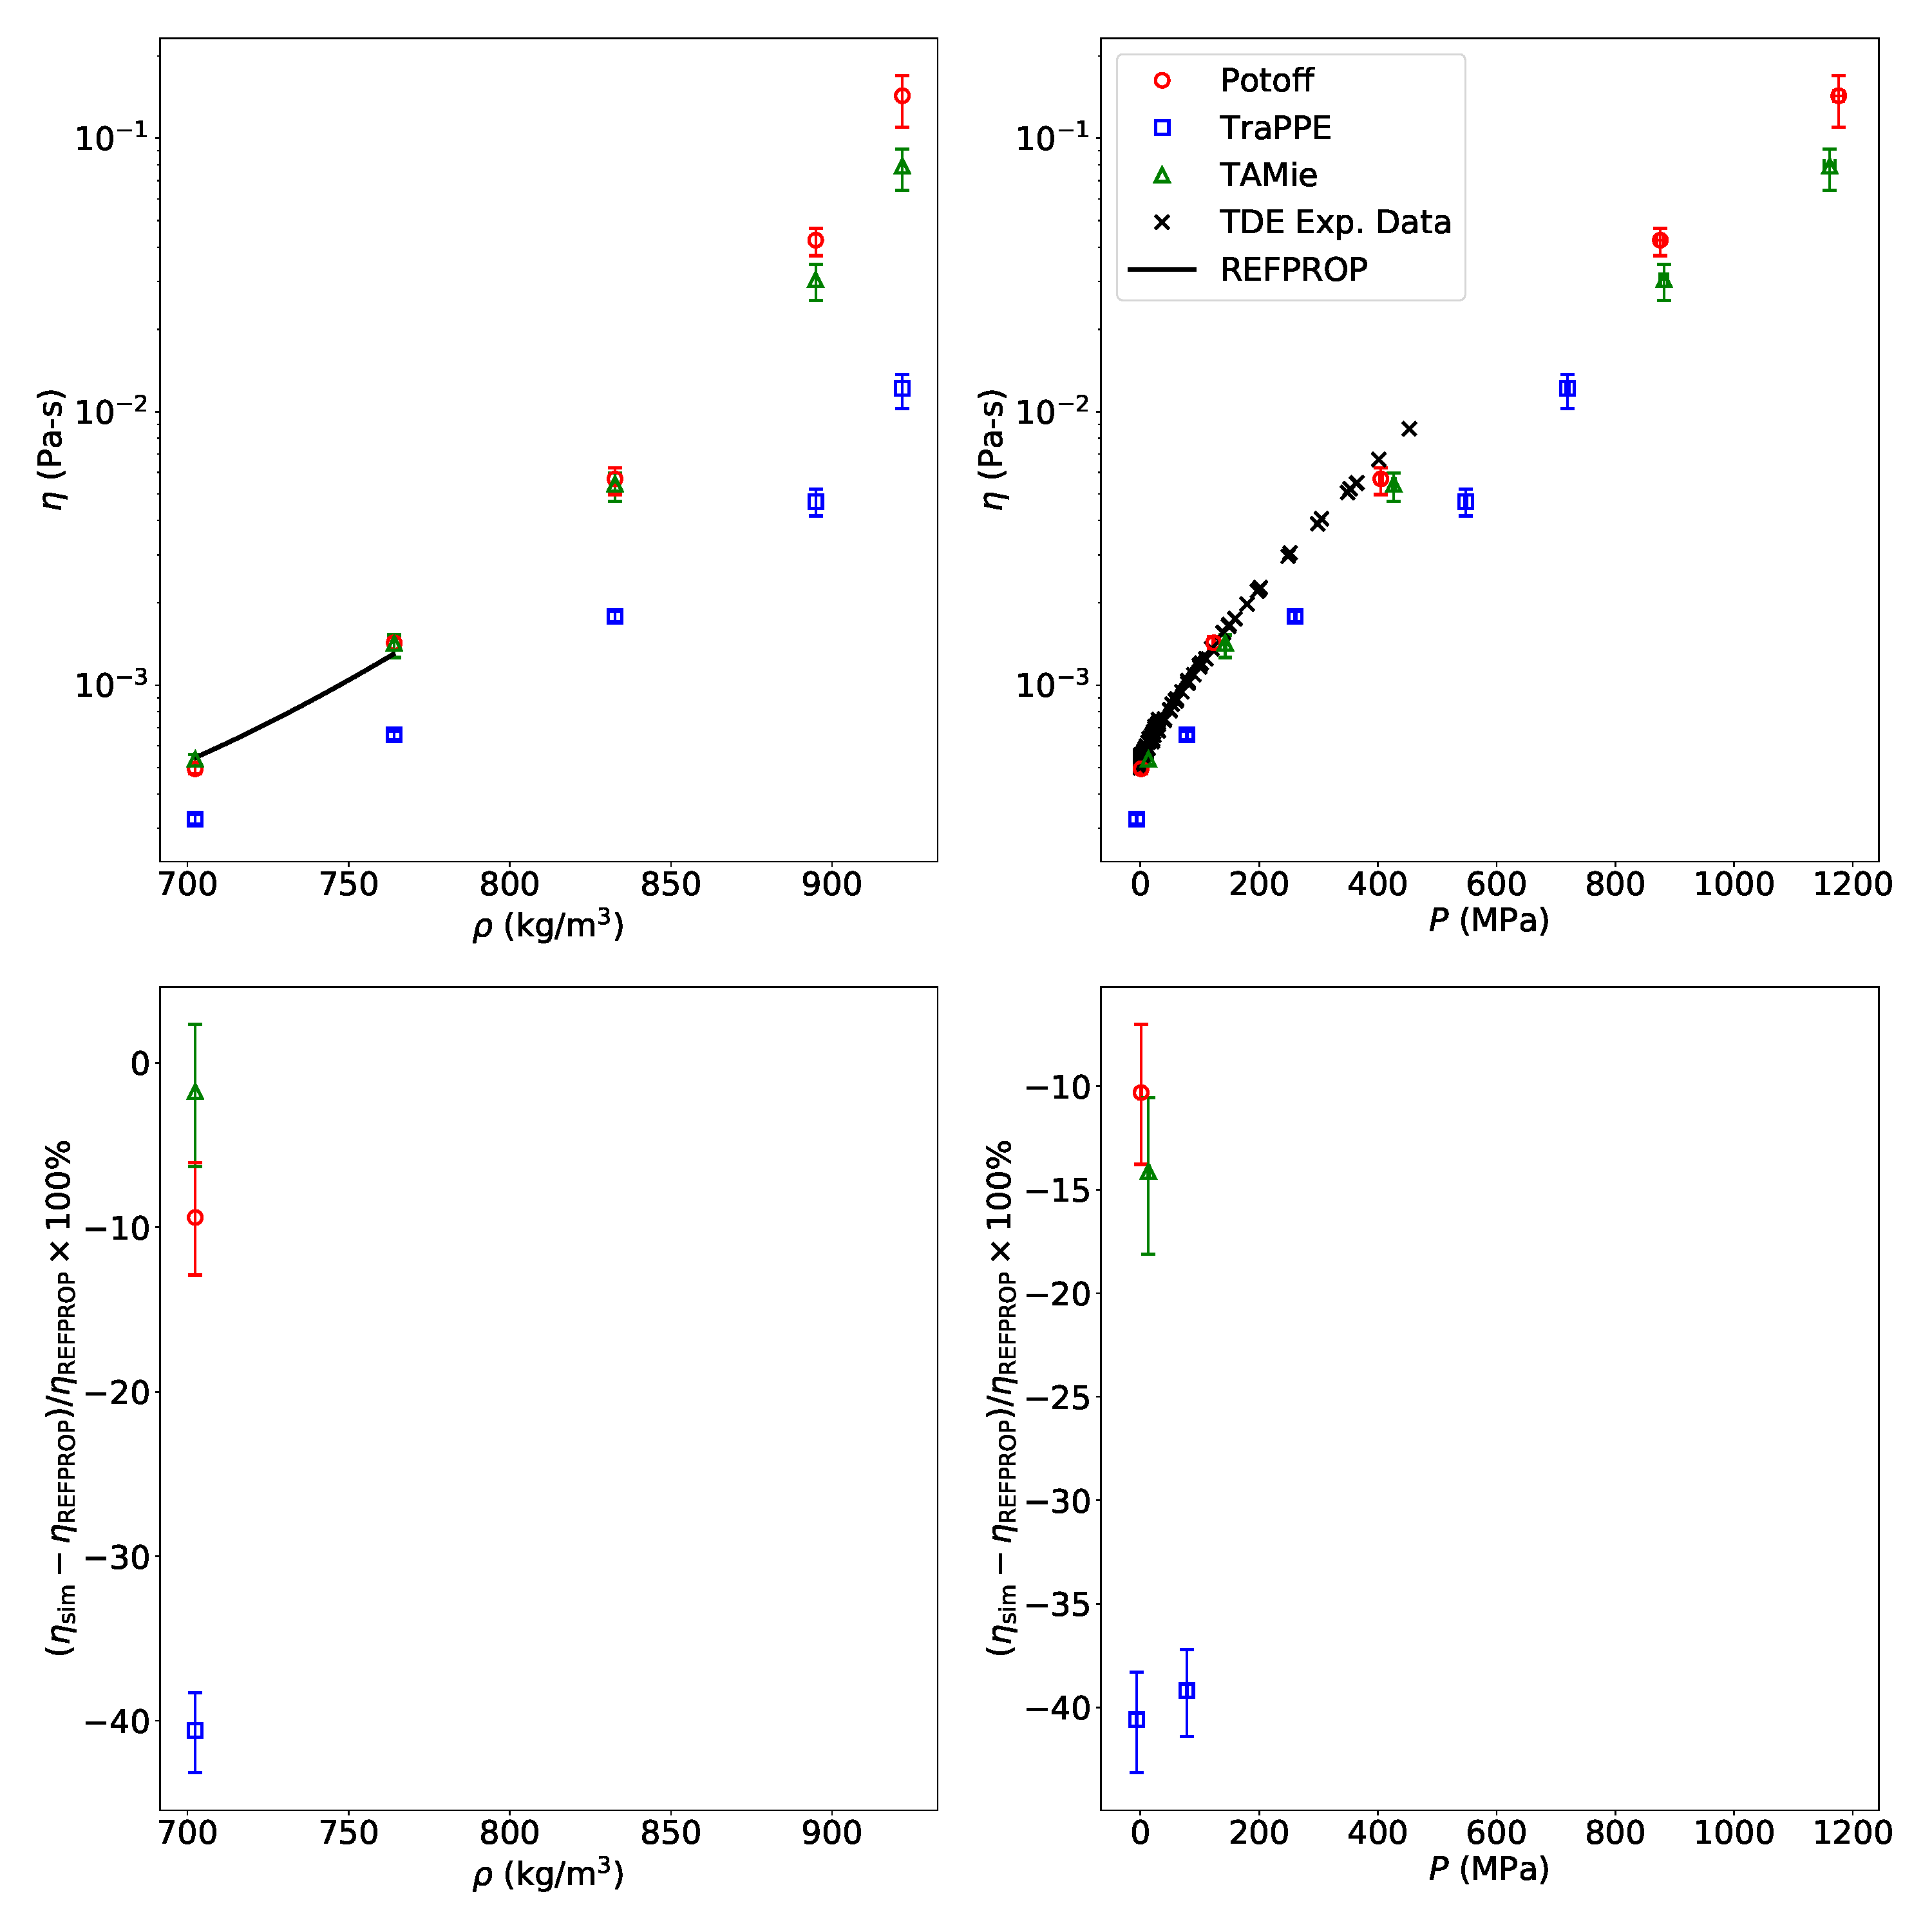
\includegraphics[width=6.4in]{compare_REFPROP_T293highP_C8H18_all.pdf}
		\caption{High density fluid viscosities at 293 K for \textit{n}-octane. Colors/symbols denote different force fields.}
		\label{fig:T293highP_C8}
	\end{figure} 
	
	\subsubsection{Branched alkanes}
	
	\begin{enumerate}
		\item Similar to n-alkanes? 
		\item Wrong torsions matters?
	\end{enumerate}
	
	%Figures:
	%
	%\begin{enumerate}
	%	\item Isobutane $\eta-\rho$ $\eta-P$
	%	\item Isopentane $\eta-\rho$ $\eta-P$
	%	%	\item Isohexane $\eta-\rho$ $\eta-P$?
	%	\item Isooctane $\eta-\rho$ $\eta-P$
	%	%	\item Neopentane $\eta-\rho$ $\eta-P$?
	%	\item 3-methylpentane $\eta-\rho$ $\eta-P$?
	%	%	\item 2,3-dimethylbutane $\eta-\rho$ $\eta-P$?
	%\end{enumerate}
	
	\begin{figure}[p!]
		\centering
		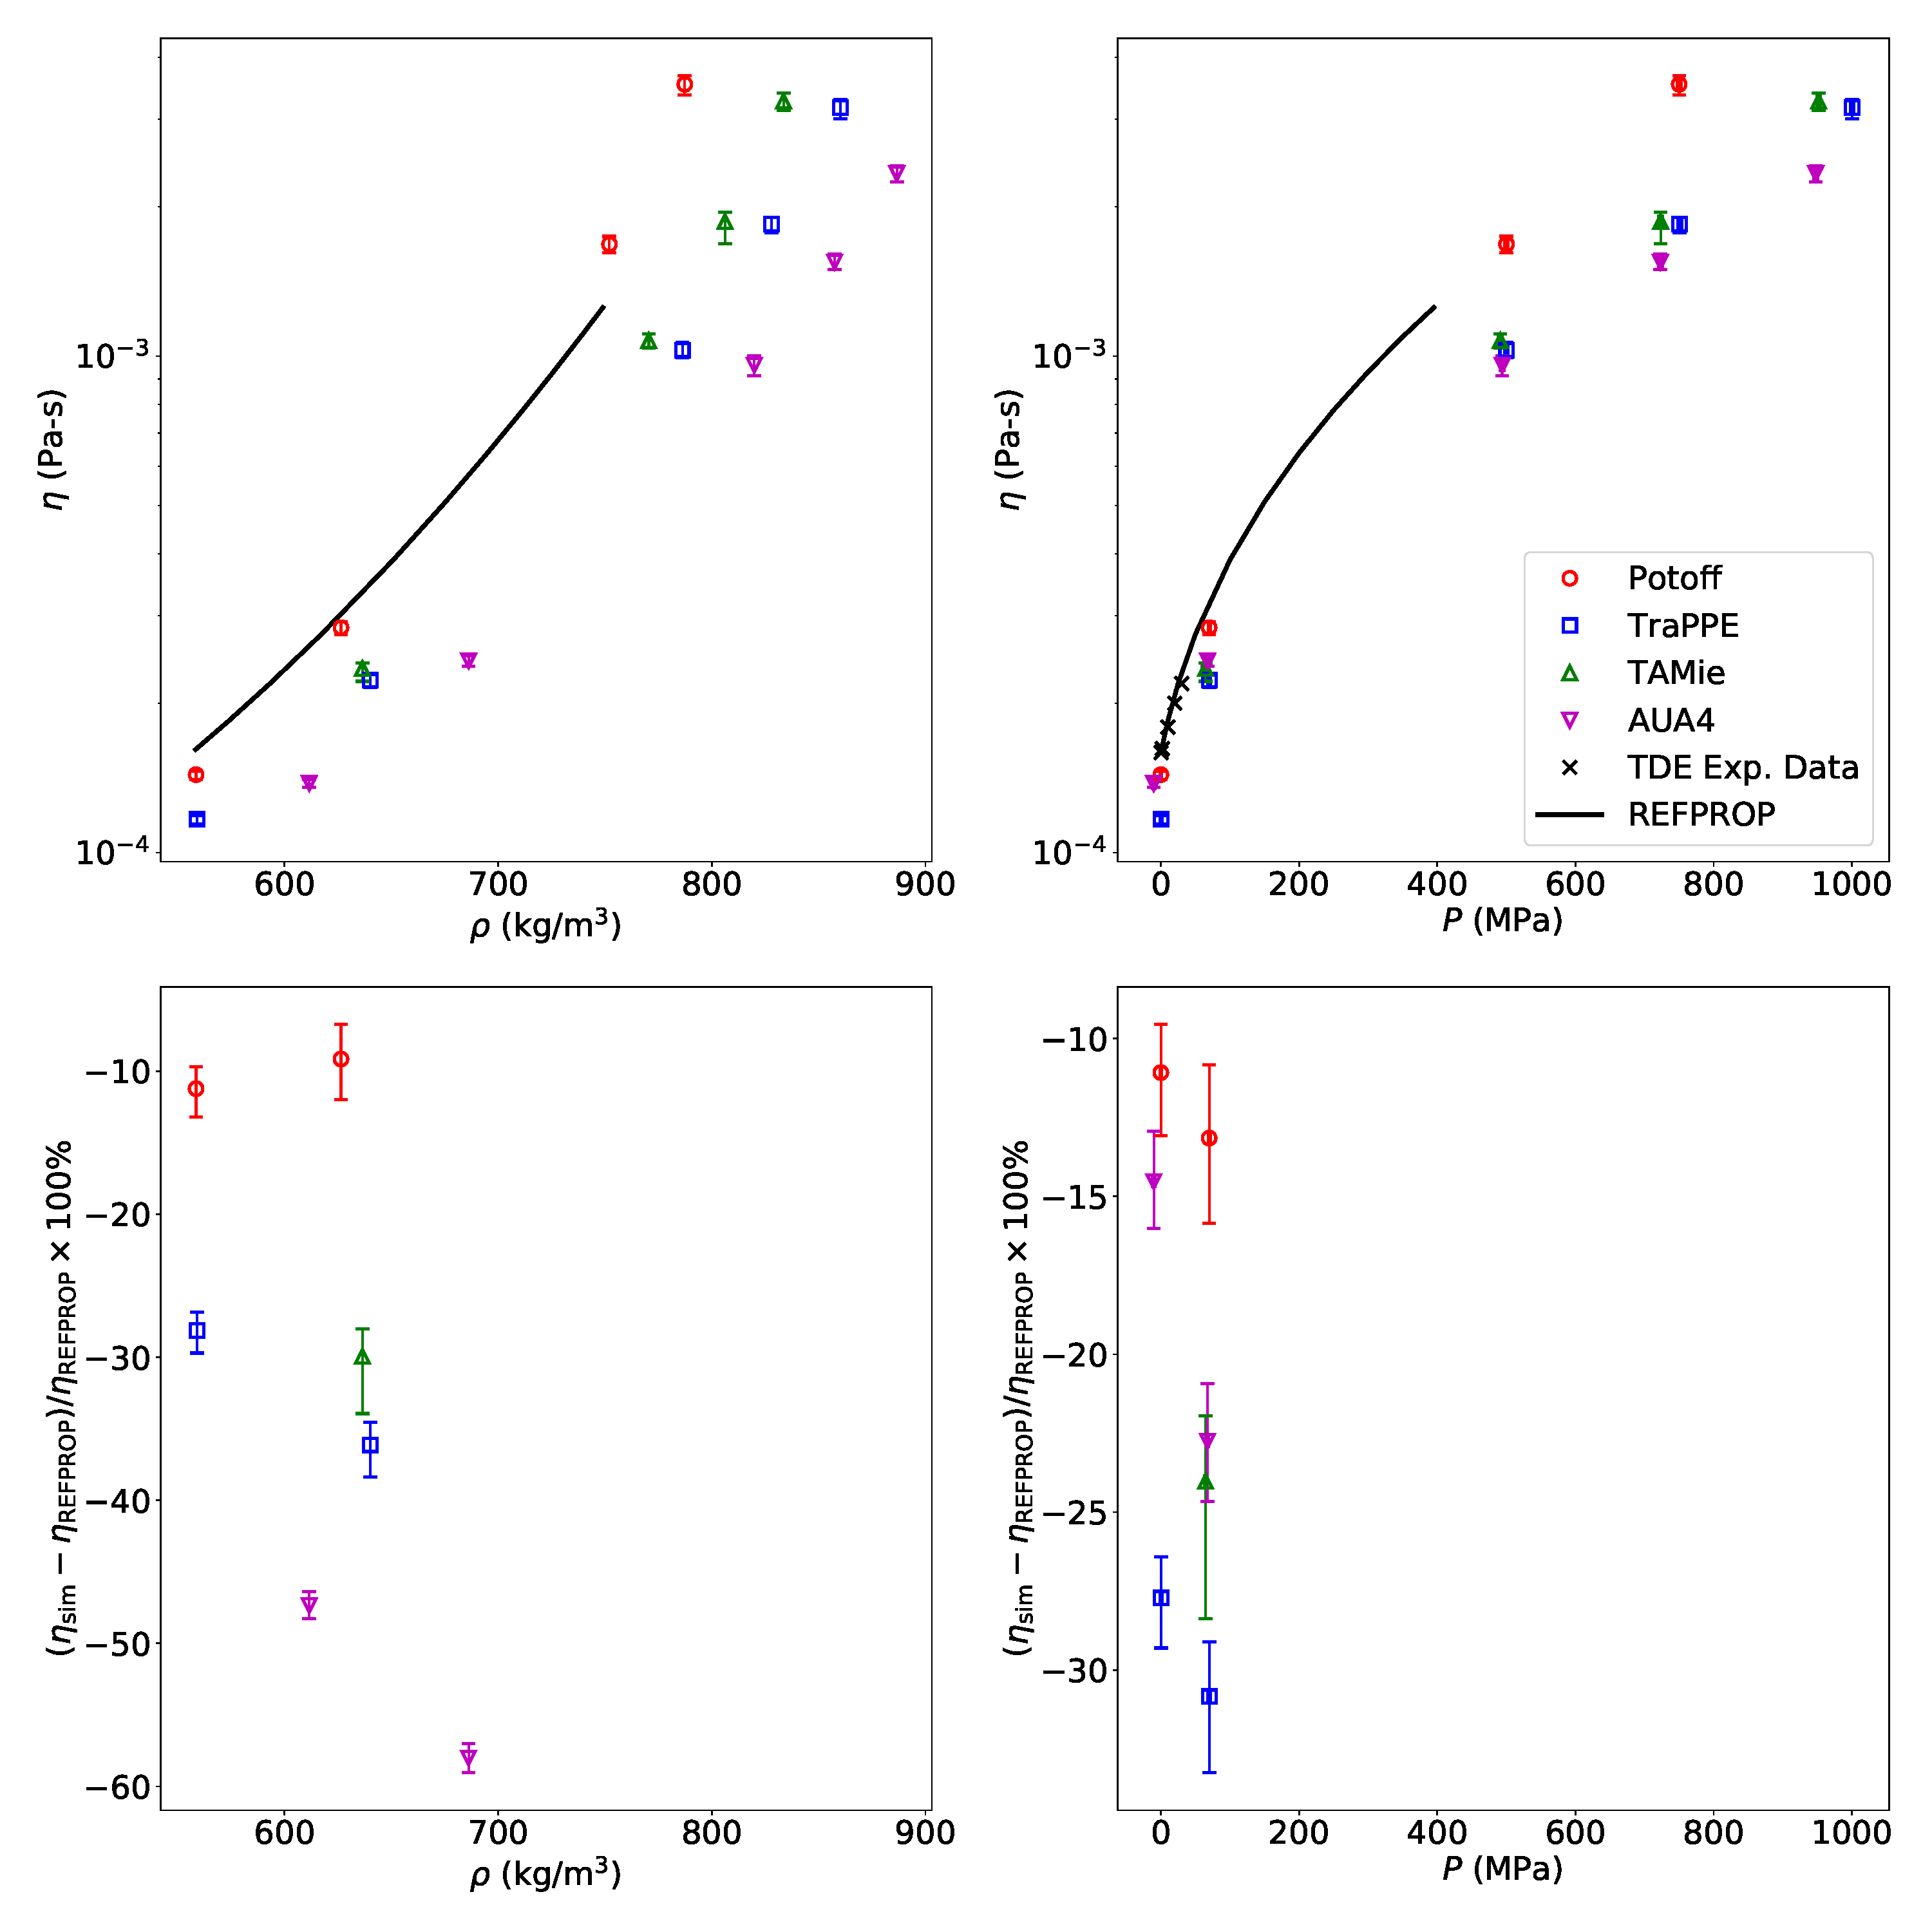
\includegraphics[width=6.4in]{compare_REFPROP_T293highP_IC4H10.pdf}
		\caption{High density fluid viscosities at 293 K for 2-methylpropane. Colors/symbols denote different force fields.}
		\label{fig:T293highP_IC4}
	\end{figure} 
	
	\begin{figure}[p!]
		\centering
		
\includegraphics[width=6.4in]{empty_figure.jpg}
		\caption{High density fluid viscosities at 293 K for 2-methylbutane. Colors/symbols denote different force fields.}
		\label{fig:T293highP_IC5}
	\end{figure} 
	
	\begin{figure}[p!]
		\centering
		
\includegraphics[width=6.4in]{empty_figure.jpg}
		\caption{High density fluid viscosities at 293 K for 3-methylpentane. Colors/symbols denote different force fields.}
		\label{fig:T293highP_3MP}
	\end{figure} 
	
	\begin{figure}[p!]
		\centering
		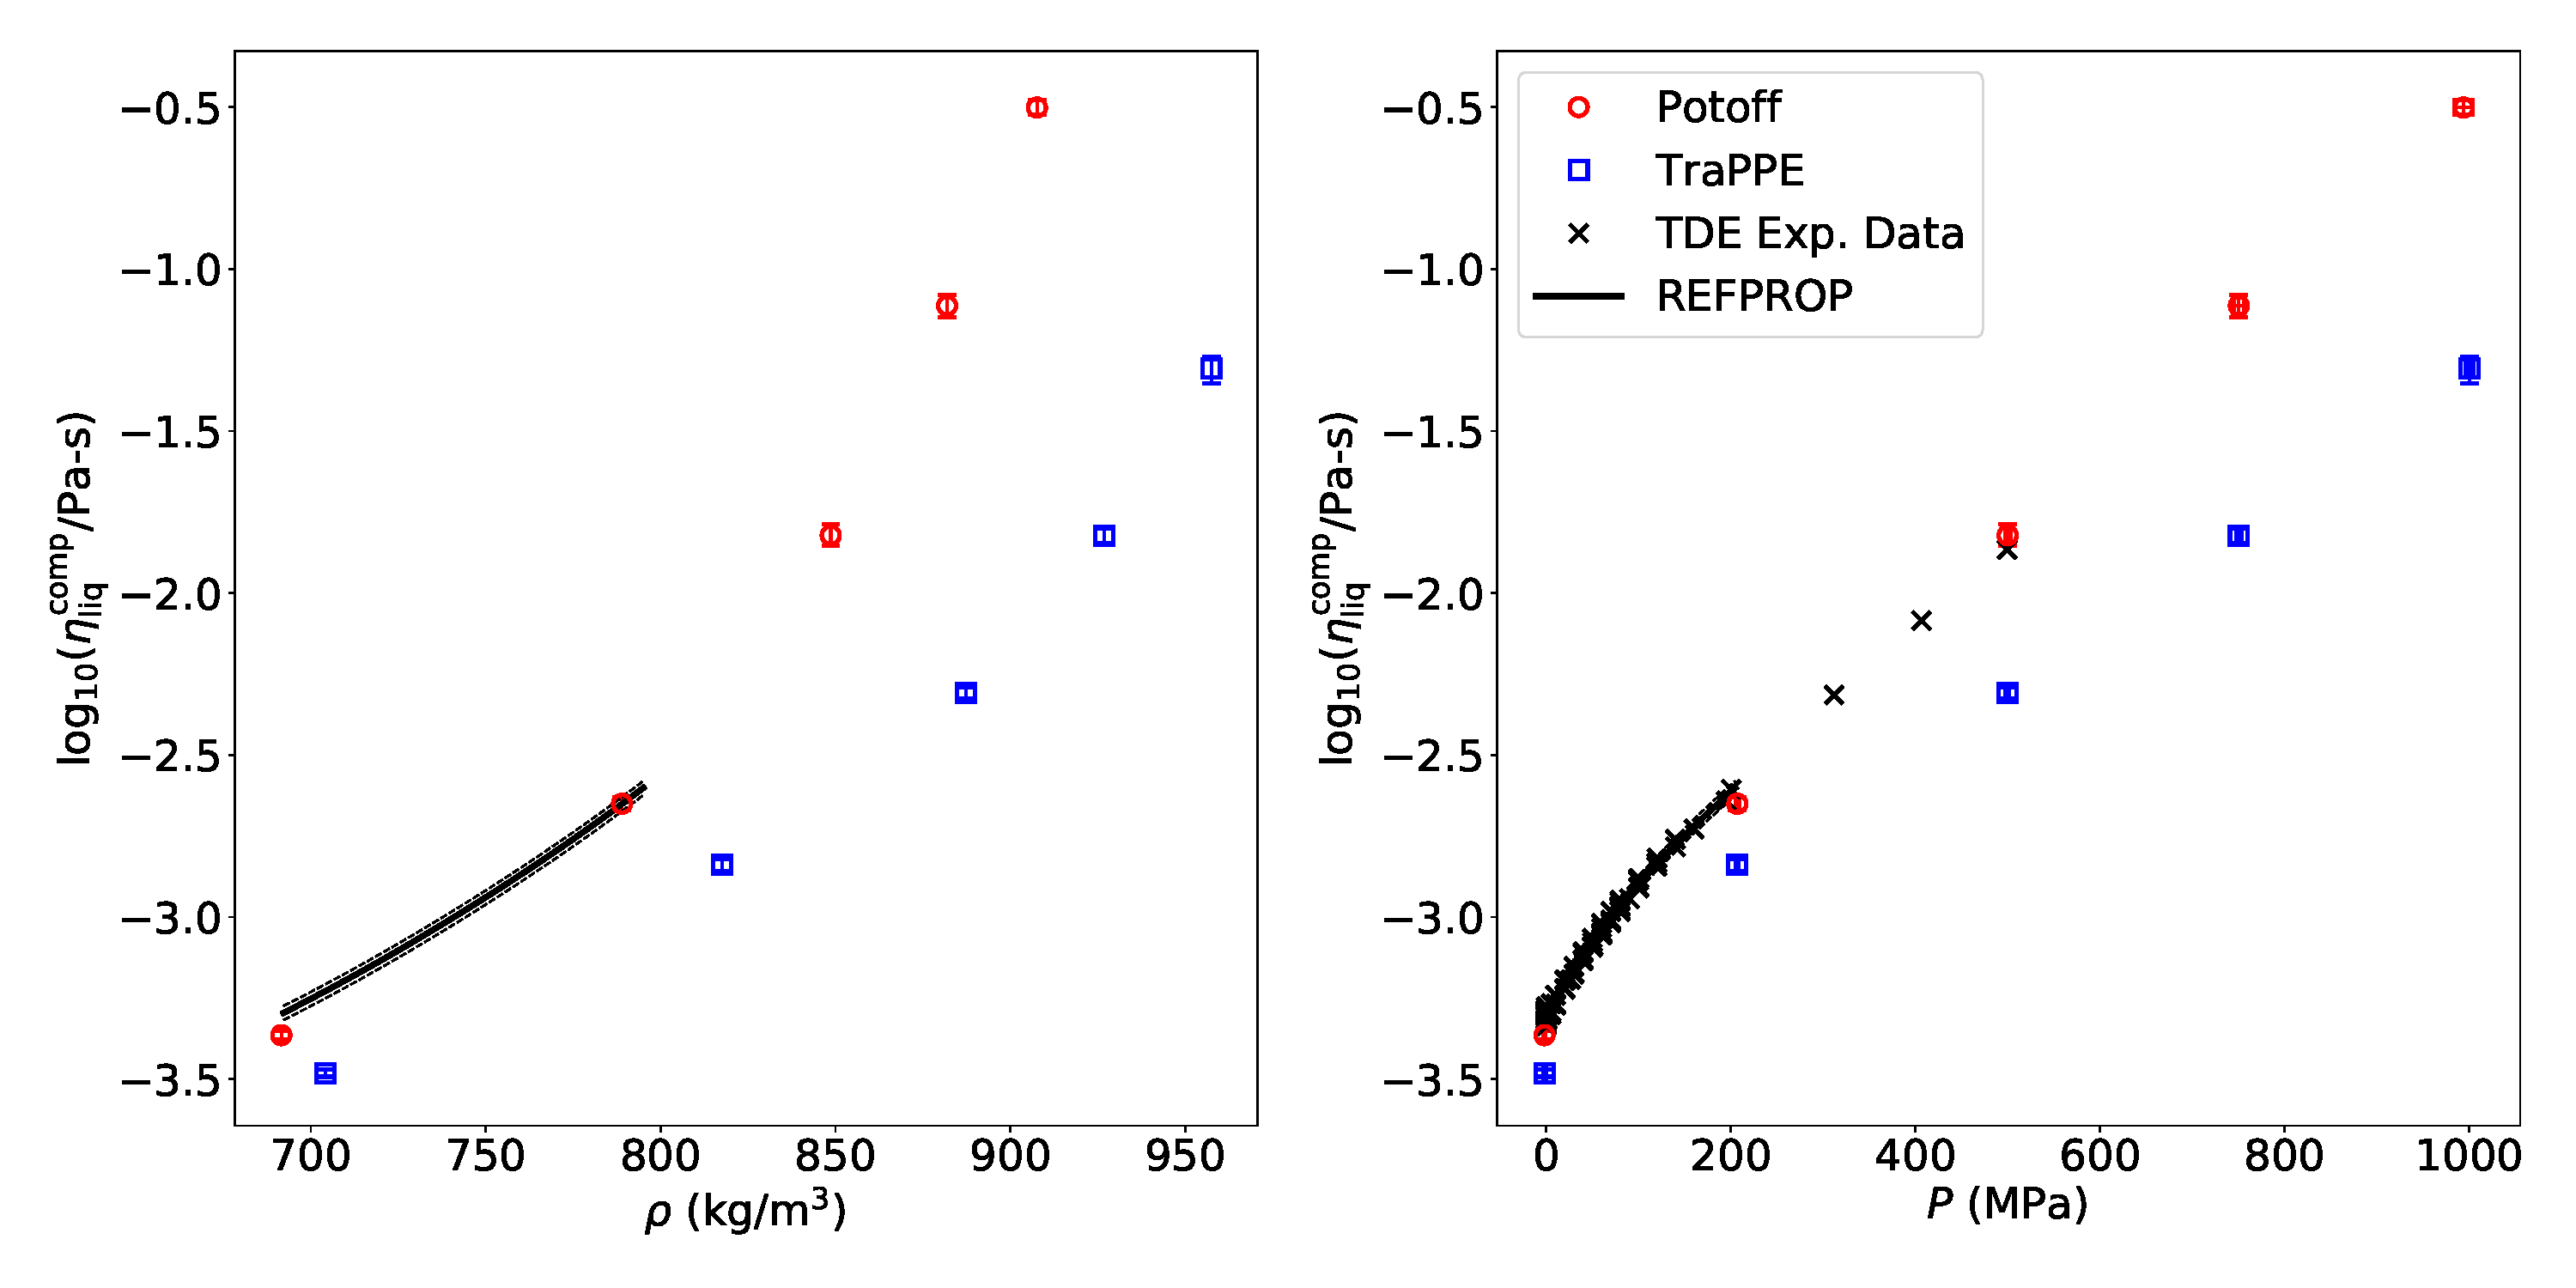
\includegraphics[width=6.4in]{compare_REFPROP_T293highP_IC8H18.pdf}
		\caption{High density fluid viscosities at 293 K for 2,2,4-trimethylpentane. Colors/symbols denote different force fields.}
		\label{fig:T293highP_IC8}
	\end{figure} 
	
	\section{Discussion/Limitations}
	
	\begin{enumerate}
		\item Discussion
		\begin{enumerate}
			\item Mie potentials parameterized with VLE data provide significant improvement over LJ 12-6
			\item Potoff over-predicts $\eta-\rho$ dependence while TAMie is fairly accurate
			\item Potoff appears to be slightly more accurate for $\eta-P$
			\item Branched alkanes are not as accurate, perhaps assumption of transferability or torsional parameters
		\end{enumerate}
		\item Limitations
		\begin{enumerate}
			\item Largest viscosity simulations are slow to converge and unclear if simulations are sufficiently long
			\item Tail-corrections could impact dynamics
			\item Using REFPROP saturation conditions instead of force fields
		\end{enumerate}
	\end{enumerate}
	
	\section{Conclusions}
	
	\section*{Acknowledgments}
	
	We are grateful for the internal review provided by NIST BERB Reviewer 1 and NIST BERB Reviewer 2 from the National Institute of Standards and Technology (NIST). 
	
	This research was performed while Richard A. Messerly held a National Research Council (NRC) Postdoctoral Research Associateship at NIST and while Michelle C. Anderson held a Summer Undergraduate Research Fellowship (SURF) position at NIST.
	
	\bibliography{Special_issue_references}
	
	\section{Supporting Information}
	
	\subsection{Gromacs input files}
	
	\begin{enumerate}
		\item Include all the .gro files
		\item Include all the .top file templates
		\item Include .mdp files
		\item Or we can just include an example and then refer them to the GitHub website
	\end{enumerate}
	
	\subsection{Tabulated values}
	
	\begin{enumerate}
		\item Ethane
		\begin{enumerate}
			\item Saturation
			\begin{enumerate}
				\item Potoff
				\item TraPPE
				\item AUA4
				\item TAMie
			\end{enumerate}
			\item T293 highP
			\begin{enumerate}
				\item Potoff
				\item TraPPE
				\item AUA4
				\item TAMie
			\end{enumerate}
		\end{enumerate}
		\item Propane
		\begin{enumerate}
			\item Saturation
			\begin{enumerate}
				\item Potoff
				\item TraPPE
				\item AUA4
				\item TAMie
			\end{enumerate}
			\item T293 highP
			\begin{enumerate}
				\item Potoff
				\item TraPPE
				\item AUA4
				\item TAMie
			\end{enumerate}
		\end{enumerate}
		\item n-Butane
		\begin{enumerate}
			\item Saturation
			\begin{enumerate}
				\item Potoff
				\item TraPPE
				\item AUA4
				\item TAMie
			\end{enumerate}
			\item T293 highP
			\begin{enumerate}
				\item Potoff
				\item TraPPE
				\item AUA4
				\item TAMie
			\end{enumerate}
		\end{enumerate}
		Repeat for all other compounds with corresponding potentials    
	\end{enumerate}
	
	\subsection{Finite-size effects}
	
	\begin{enumerate}
		\item Simulation results for 100, 200, 400, and 800 molecules
	\end{enumerate}
	
	\subsection{Simulation length effects}
	
	\begin{enumerate}
		\item Verified that 1 ns is long enough for larger compounds
	\end{enumerate}
	
	\subsection{Validation Runs}
	
	\begin{enumerate}
		\item Ethane NIST
		\item n-Octane Literature
	\end{enumerate}
	
	\subsection{Bond types, Harmonic vs LINCS}
	
	\begin{enumerate}
		\item Propane and n-butane with harmonic (arbirary bond constant) shows systematic increase
	\end{enumerate}
	
	\subsection{Green-Kubo analysis}
	
	\begin{enumerate}
		\item Raw data, i.e., multiple replicates with the average
		\item Exclude low time data and have a heurestic for determining the cut-off time
	\end{enumerate}
	
	Example analysis, i.e., bootstrap distribution, replicates
	
	\subsection{MCMC?}
	
	
	
	
\end{document}
